\documentclass[10pt,show notes on second screen]{beamer}

\usepackage{appendixnumberbeamer}
\usepackage[numbers,sort&compress]{natbib}
\usepackage{amsfonts}
\usepackage{amsmath}
\usepackage{mathtools}
\usepackage{amssymb}
\usepackage{mathrsfs}
\usepackage{units}

% For LatViz animations
\usepackage{animate}

% For nice algoritms
\usepackage{algorithm}
\usepackage{algorithmicx}
\usepackage{algpseudocode}

% For coloring equations
\usepackage{color}
\makeatletter
\def\mathcolor#1#{\@mathcolor{#1}}
\def\@mathcolor#1#2#3{%
\protect\leavevmode\begingroup\color#1{#2}#3\endgroup}
\makeatother

% % For proper referencing
\usepackage{varioref}
\usepackage{hyperref}
\hypersetup{
    breaklinks={true},
}
\usepackage{cleveref}

% For writing C++ in listings
\usepackage{listings}
\lstset{language=C++,
        basicstyle=\ttfamily,
        keywordstyle=\color{blue}\ttfamily,
        stringstyle=\color{red}\ttfamily,
        commentstyle=\color{green}\ttfamily,
        morecomment=[l][\color{magenta}]{\#}
}

% For including sub figures
\usepackage{subcaption}

% For nice tables
\usepackage{booktabs}

% For figures and graphics'n stuff
\usepackage{graphicx}
\usepackage{caption}

% \usetheme[progressbar=frametitle]{metropolis}
\usetheme{metropolis}

% For notes
\usepackage{pgfpages}
\setbeamertemplate{note page}[plain]
\setbeameroption{show notes on second screen=bottom}

\usefonttheme[onlymath]{serif}

% Titles, date, ect.
\title{Solving \texorpdfstring{$\SU(3)$}{SU3} Yang-Mills theory on the lattice: a calculation of selected gauge observables with gradient flow}
\date{\today}
\author{Hans Mathias Mamen Vege}
\institute{University of Oslo}

\bibliographystyle{plainnat}

% Loads command list
% For Feynman slashes
\usepackage{slashed}

\newcommand{\husk}[1]{\color{red}#1\color{black}}
\newcommand{\TODO}[1]{\color{red}#1\color{black}}
\newcommand{\expect}[1]{\left\langle{#1}\right\rangle}
\newcommand{\Tr}{\mathrm{Tr}}
\newcommand{\tr}{\mathrm{tr}}
\newcommand{\dd}{\mathrm{d}}
\newcommand{\e}{\mathrm{e}}
\newcommand{\SU}{\mathrm{SU}}
\newcommand{\conj}[1]{\overline{#1}}
\newcommand{\sign}{\mathrm{sign}}
\newcommand{\epsrnd}{\varepsilon_\mathrm{rnd}}

% For fermi units
\newcommand{\fm}{\mathrm{fm}}

% Complex number notation
\renewcommand{\Re}{\operatorname{Re}}
\renewcommand{\Im}{\operatorname{Im}}

% Commands for writing shorthand lattice operators
\newcommand{\MU}{\hat{\mu}}
\newcommand{\NU}{\hat{\nu}}

\renewcommand{\vec}[1]{\boldsymbol{\mathbf{#1}}}
% BEGIN COMMANDS FROM LATEX FOR PHYSICISTS
% http://www.dfcd.net/articles/latex/latex.html
\newcommand{\ket}[1]{\left| #1 \right\rangle} % for Dirac bras
\newcommand{\bra}[1]{\left\langle #1 \right|} % for Dirac kets
\newcommand{\bket}[1]{\right| #1 \right\rangle} % for Dirac bras
\newcommand{\bbra}[1]{\left\langle #1 \left|} % for Dirac kets

% Front page
\setbeamertemplate{title page}{
    \begin{minipage}[c][\paperheight]{\textwidth}
        \ifx\inserttitlegraphic\@empty\else\usebeamertemplate*{title graphic}\fi
        \vfill%
        {
        \centering
        \ifx\inserttitle\@empty\else\usebeamertemplate*{title}\fi
        \ifx\insertsubtitle\@empty\else\usebeamertemplate*{subtitle}\fi
        }
        \usebeamertemplate*{title separator}
        \begin{minipage}[t]{.4\textwidth}
            \ifx\beamer@shortauthor\@empty\else\usebeamertemplate*{author}\fi
            \ifx\insertdate\@empty\else\usebeamertemplate*{date}\fi
        \end{minipage}
        \begin{minipage}[t]{.6\textwidth}
            \vspace*{2em}
            {\hspace{1.2em}\small Supervisor: \textit{Andrea Shindler} \par}
            \vspace*{0.2em}
            {\hspace{1.2em}\small Co-supervisor: \textit{Morten Hjorth-Jensen}}
        \end{minipage}%

        \begin{minipage}[t]{\textwidth}
            \centering
            \ifx\insertinstitute\@empty\else\usebeamertemplate*{institute}\fi
        \end{minipage}
        \vfill
        \vspace*{1mm}
    \end{minipage}
}



\newcommand{\CC}{C\nolinebreak\hspace{-.05em}\raisebox{.4ex}{\tiny\bf +}\nolinebreak\hspace{-.10em}\raisebox{.4ex}{\tiny\bf +}}
\def\CC{{C\nolinebreak[4]\hspace{-.05em}\raisebox{.4ex}{\tiny\bf ++ }}}

% For aligned undersets
\usepackage{stackengine}
\def\stacktype{L}
\setstackgap{L}{1.2\normalbaselineskip}
\stackMath
\tabularnewline

\begin{document}

\setbeamercolor{background canvas}{bg=white}
\maketitle

% \begin{frame}{Structure}
%   % \setbeamertemplate{section in toc}[sections numbered]
%   \tableofcontents[hideallsubsections]
% \end{frame}

%%%%%%%%%%%%%%%%%%%%%%%%%%%%%%%%%%%%%%%%%%%%%%%%%%%%%%%%%%%%%%%%%%%%%%%%%%%%%%%%%%%%%%%%%%
%  ___       _                 _            _   _
% |_ _|_ __ | |_ _ __ ___   __| |_   _  ___| |_(_) ___  _ __
%  | || '_ \| __| '__/ _ \ / _` | | | |/ __| __| |/ _ \| '_ \
%  | || | | | |_| | | (_) | (_| | |_| | (__| |_| | (_) | | | |
% |___|_| |_|\__|_|  \___/ \__,_|\__,_|\___|\__|_|\___/|_| |_|
%%%%%%%%%%%%%%%%%%%%%%%%%%%%%%%%%%%%%%%%%%%%%%%%%%%%%%%%%%%%%%%%%%%%%%%%%%%%%%%%%%%%%%%%%%
\section{Introduction}

\begin{frame}{Structure}
    \begin{itemize}[<+->]
        \item Quantum Chromodynamics(QCD).
        \item Lattice QCD.
        \item Gradient flow.
        \item Developing a code for solving $\SU(3)$ Yang-Mills theory.
        \item Results.
    \end{itemize}
    \note{
    \begin{itemize}[<+->]
        \item \textbf{QCD.} We will go through and explain what QCD as well as motivate its existence.
        \item \textbf{LQCD.} We will briefly show how one discretise the lattice and perform calculations on it.
        \item \textbf{Gradient flow.} We will quickly introduce gradient flow and explain its effects.
        \item \textbf{GLAC.} Will briefly present the code which we developed as well as some benchmarks. We will also present the Metropolis algorithm.
        \item \textbf{Results.} We will present the results obtained from pure gauge calculations.
    \end{itemize}
    }
\end{frame}

%%%%%%%%%%%%%%%%%%%%%%%%%%%%%%%%%%%%%%%%%%%%%%%%%%%%%%%%%%%%%%%%%%%%%%%%%%%%%%%%%%%%%%%%%%
%   ___   ____ ____
%  / _ \ / ___|  _ \
% | | | | |   | | | |
% | |_| | |___| |_| |
%  \__\_\\____|____/
%%%%%%%%%%%%%%%%%%%%%%%%%%%%%%%%%%%%%%%%%%%%%%%%%%%%%%%%%%%%%%%%%%%%%%%%%%%%%%%%%%%%%%%%%%
\section{Quantum Chromodynamics(QCD)}

% \begin{frame}{QCD}
% \begin{itemize}[<+->]
%     \item The standard model: Six quarks and eight gluons
%     \item Asymptotic freedom
%     \item Confinement
%     \item Highly nonlinear due to gluon self-interactions
% \end{itemize}
% \note{
% \begin{itemize}[<+->]
%     \item \textbf{The standard model.} 
%     \item \textbf{Asymptotic freedom.} 
%     \item \textbf{Confinement.} 
%     \item \textbf{Nonlinearity.} 
% \end{itemize}
% }
% \end{frame}

\begin{frame}{The Standard Model}
    \begin{center}
        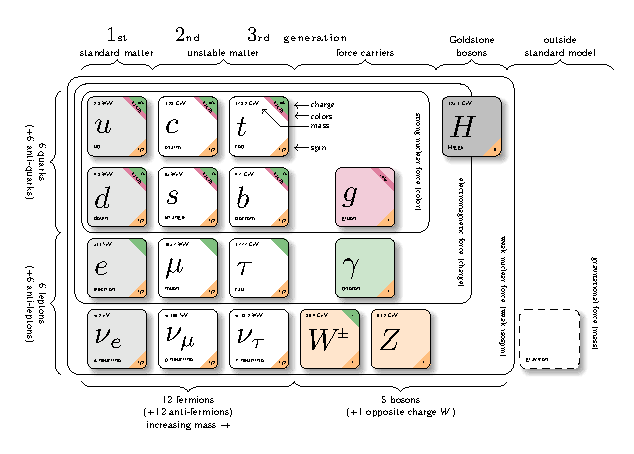
\includegraphics[width=0.8\textwidth]{../figures/illustrations/qcd/standard-model/sm.pdf}
    \end{center}
    \note{Consists of the innermost square of the \textbf{six quarks} and the \textit{eight gluons}.}
\end{frame}

\begin{frame}{The non-linearity of QCD}
The QCD Lagrangian
\begin{align*}
    \mathcal{L}_\mathrm{QCD} = \sum^{N_f}_{f=1} \bar{\psi}^{(f)} \left(i\slashed{D} - m^{(f)}\right) \psi^{(f)} - \frac{1}{4}G^a_{\mu\nu}G^{a\mu\nu},
\end{align*}
with action
\begin{align}
    S = \int \dd^4 x \mathcal{L}_\mathrm{QCD},
\end{align}
is invariant under a $\SU(3)$ symmetry.

\begin{align*}
    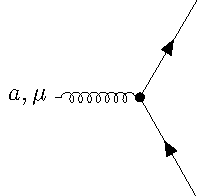
\includegraphics[scale=0.9]{../figures/feynman-diagrams/fermion-gluon-vertex/fermion-gluon-vertex.pdf} \quad
    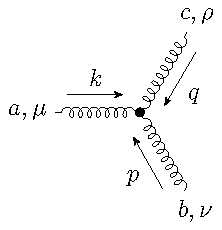
\includegraphics[scale=0.9]{../figures/feynman-diagrams/three-gluon-vertex/three-gluon-vertex.pdf} \quad
    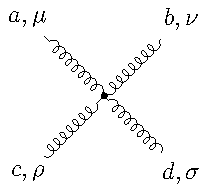
\includegraphics[scale=0.9]{../figures/feynman-diagrams/four-gluon-vertex/four-gluon-vertex.pdf}
\end{align*}
\note{
    \begin{itemize}
        \item \textit{Gluon self-interaction.}
        \item This central aspect is mostly covered in the pure-gauge/Yang-Mills section of the theory.
        \item \textbf{Two important features}: \textit{confinement} and \textit{asymptotic freedom}.
    \end{itemize}
}
\end{frame}

\begin{frame}{Asymptotic freedom}
    \begin{center}
        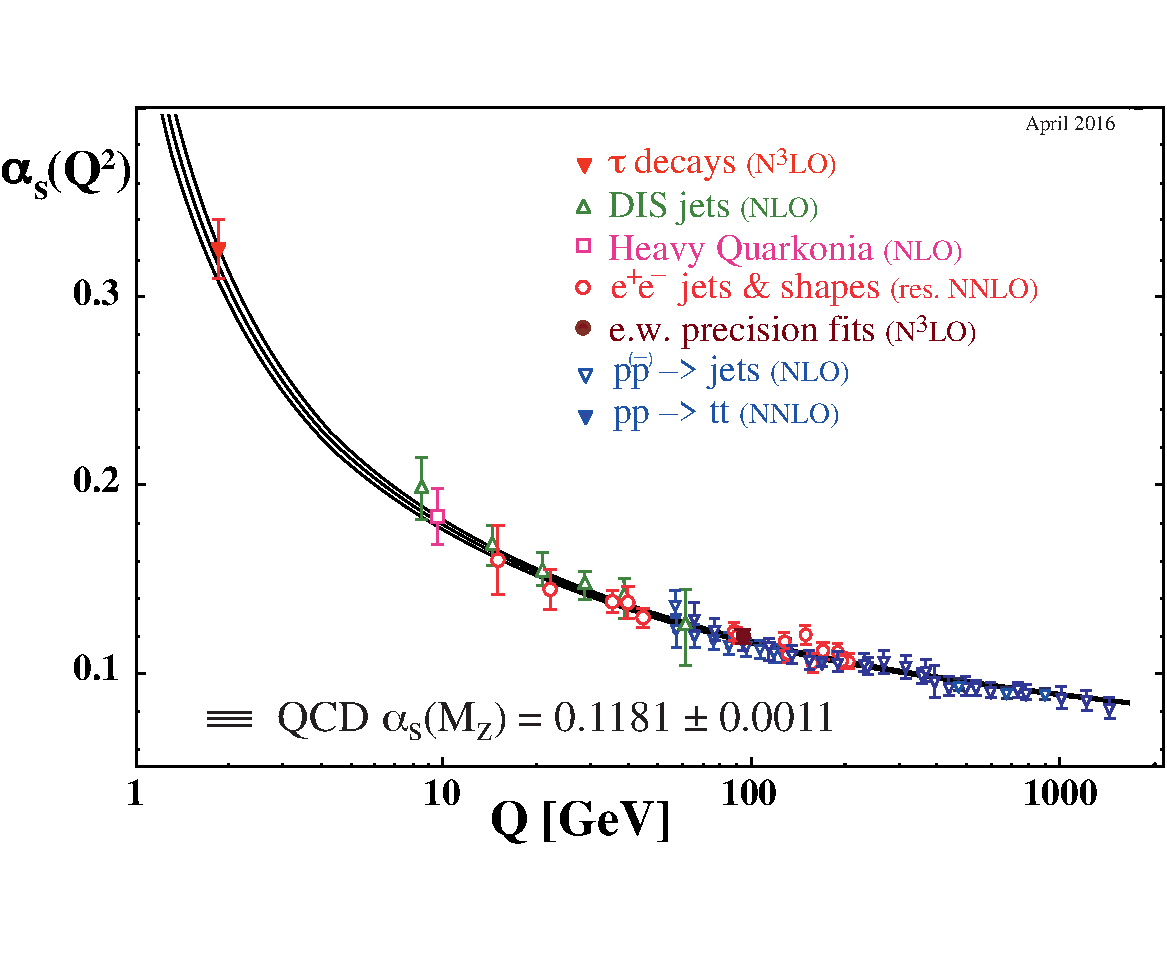
\includegraphics[width=0.8\textwidth]{../figures/pdg_asymptotic_freedom-eps-converted-to.pdf}
    \end{center}
    \note{
        \begin{itemize}
            \item The coupling constant \textbf{decreases} as we \textbf{increase} the energy.
            \item Also serves as an \textit{experimental proof} of QCD.
            \item Other lines of \textit{evidence}: triple $\gamma$ decay and muon cross section ratio $R$.
            \begin{itemize}
                \item Triple $\gamma$ decay: the number of colors is included in the cross section, which can be measured experimentally.
                \item Muon cross section ratio $R$: the ratio is dependent on having three colors.
            \end{itemize}
        \end{itemize}
    }
\end{frame}

\begin{frame}{Confinement}
    \begin{center}
        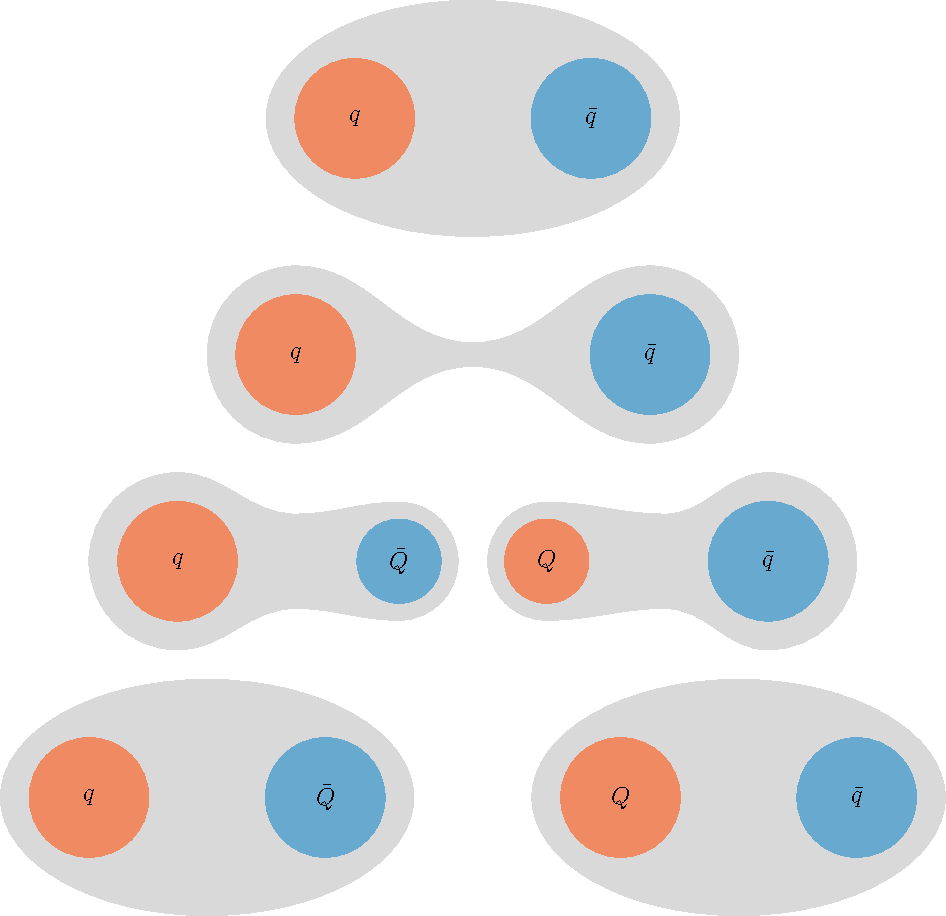
\includegraphics[width=0.65\textwidth]{../figures/illustrations/qcd/confinement/string-breaking.pdf}
    \end{center}
    \note{If we try to pull apart \textbf{two quarks in a meson}, more and more energy is required until we have enough energy to spontaneously create a \textbf{quark-antiquark} pair, forming thus \textbf{two new mesons.}}
\end{frame}

%%%%%%%%%%%%%%%%%%%%%%%%%%%%%%%%%%%%%%%%%%%%%%%%%%%%%%%%%%%%%%%%%%%%%%%%%%%%%%%%%%%%%%%%%%
%  _          _   _   _             ___   ____ ____
% | |    __ _| |_| |_(_) ___ ___   / _ \ / ___|  _ \
% | |   / _` | __| __| |/ __/ _ \ | | | | |   | | | |
% | |__| (_| | |_| |_| | (_|  __/ | |_| | |___| |_| |
% |_____\__,_|\__|\__|_|\___\___|  \__\_\\____|____/
%%%%%%%%%%%%%%%%%%%%%%%%%%%%%%%%%%%%%%%%%%%%%%%%%%%%%%%%%%%%%%%%%%%%%%%%%%%%%%%%%%%%%%%%%%
\section{Lattice Quantum Chromodynamics(LQCD)}

\begin{frame}{Discretizing spacetime}
\begin{block}{}
\begin{enumerate}
    \item <1->Divide spacetime into a cube of size $N^3\times N_T$.
    \item <2->Fermions live on the each \textit{point} in the cube.
    \item <3->The gauge fields live on the sites \textit{in between} the points, and is called links.
\end{enumerate}
\end{block}
\onslide<4->{Goal: \textit{maintain gauge invariance.}}
\note{Make a quick drawing perhaps of a lattice?}
\end{frame}

\begin{frame}{Links}
% \begin{align*}
%     U_\mu(n) = \exp \left[ i a A_\mu (n) \right],
% \end{align*}
A link connects one lattice site to another and is a $\SU(3)$ matrix.
\begin{figure}
    \centering
    \begin{subfigure}{0.48\textwidth}
        \centering
        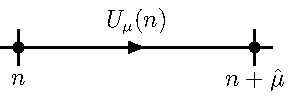
\includegraphics{../figures/illustrations/lqcd/links/link}
        \label{fig:lqcd:link}
    \end{subfigure}
    \begin{subfigure}{0.48\textwidth}
        \centering
        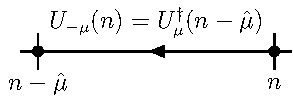
\includegraphics{../figures/illustrations/lqcd/links/link-inverse}
        \label{fig:lqcd:link-inverse}
    \end{subfigure}
    \centering
\end{figure}
where $U_{-\mu}(n) = U_\mu(n - \hat{\mu})^\dagger$.
\note{
    \begin{itemize}
        \item Defined from the gauge transporter.
        \item A link in the positive $\MU$ direction is shown in the figure to the left.
        \item A link in the negative $\MU$ direction is shown in the figure to the right.
    \end{itemize}
}
\end{frame}

\begin{frame}{Gauge invariance on the lattice} %\husk{TODO: Don't need to show the gauge transformation!?}
\begin{block}
    \only<1->{Links constructed such that we maintain gauge invariance in the action,}
    \only<2->{\begin{align*}
            U_\mu(n) &\rightarrow U_\mu'(n) = \Omega(n) U_\mu(n) \Omega(n+\hat{\mu})^\dagger, \\
            U_{-\mu}(n) &\rightarrow U_{-\mu}'(n) = \Omega(n) U_{\mu}(n-\hat{\mu})^\dagger \Omega(n-\hat{\mu})^\dagger.
        \end{align*}}
    \only<3->{Two main types of gauge invariant objects,}
    \begin{itemize}
        \item<4-> Objects with fermions $\psi$, $\bar{\psi}$ as end points.
        \item<5-> Fully connected gauge invariant objects(i.e. ``loops'').
    \end{itemize}
\end{block}
\end{frame}

\begin{frame}{The plaquette}
The simplest gauge invariant object,
% \begin{align*}
%     P_{\mu\nu}(n) &= U_\mu(n) U_{\nu}(n+\hat{\mu}) U_{-\mu}(n+\hat{\mu}+\hat{\nu}) U_{-\nu} (n+\hat{\nu}) \nonumber \\
%     &= U_\mu(n) U_{\nu}(n+\hat{\mu}) U_{\mu}(n+\hat{\nu})^\dagger U_{\nu} (n)^\dagger,
% \end{align*}
\begin{figure}
    \centering
    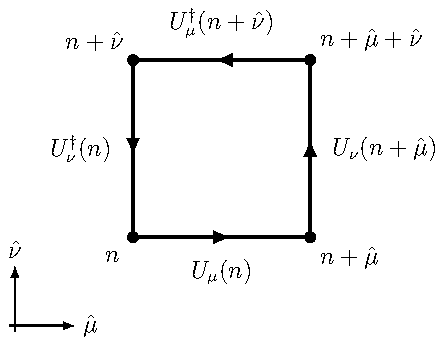
\includegraphics[scale=1]{../figures/illustrations/lqcd/plaquette/plaquette}
\end{figure}
\end{frame}

\begin{frame}{The Wilson gauge action}
The Wilson gauge action is given as
\begin{align}
    S_G[U] = \frac{\beta}{3} \sum_{n\in\Lambda} \sum_{\mu<\nu} \Re \tr \left[ 1 - P_{\mu\nu}(n) \right],
\end{align}
with $\beta=6/g_S^2$.

Continuum action recovered when $a \rightarrow 0$!
\note{
    \begin{itemize}
        \item Using the definition of the link we saw earlier, we can reproduce the continuum action up to an discretization error of $\mathcal{O}(a^2)$.
    \end{itemize}
}
\end{frame}

%%%%%%%%%%%%%%%%%%%%%%%%%%%%%%%%%%%%%%%%%%%%%%%%%%%%%%%%%%%%%%%%%%%%%%%%%%%%%%%%%%%%%%%%%%
%  ____                 _             _                                     _
% |  _ \  _____   _____| | ___  _ __ (_)_ __   __ _    __ _    ___ ___   __| | ___
% | | | |/ _ \ \ / / _ \ |/ _ \| '_ \| | '_ \ / _` |  / _` |  / __/ _ \ / _` |/ _ \
% | |_| |  __/\ V /  __/ | (_) | |_) | | | | | (_| | | (_| | | (_| (_) | (_| |  __/
% |____/ \___| \_/ \___|_|\___/| .__/|_|_| |_|\__, |  \__,_|  \___\___/ \__,_|\___|
%                              |_|            |___/
%%%%%%%%%%%%%%%%%%%%%%%%%%%%%%%%%%%%%%%%%%%%%%%%%%%%%%%%%%%%%%%%%%%%%%%%%%%%%%%%%%%%%%%%%%
\section{Developing a code for solving \texorpdfstring{$\SU(3)$}{SU3} Yang-Mills theory on the lattice}
\begin{frame}{The numerical challenge in lattice QCD}
\onslide<1->{A lattice configuration consists of $3\times 3$ $\SU(3)$ matrices,}
\onslide<2->{\begin{align*}
    \stackunder{\underbrace{N^3}}{\text{Spatial}} \times \stackunder{\underbrace{N_T}}{\text{Temporal}} \times \stackunder{\underbrace{4}}{\text{Links}} \times \stackunder{\underbrace{9}}{\text{$\SU(3)$ matrix}} \times \stackunder{\underbrace{2}}{\text{$\mathbb{C}$-numbers}} = 72 N^3N_T,
\end{align*}}
\onslide<3->{$\rightarrow 8 \times 72N^3N_T$ bytes.}
\note{
    \begin{itemize}
        \item The $\SU(3)$ matrices are $3\times 3$ matrices of nine complex numbers or 18 real numbers.
        \item This leads to an absolute \textbf{requirement of efficiency}, both in \textbf{calculations} and in \textbf{input/output}.
        \item When returning to what ensembles of configurations we generated this will be evident.
    \end{itemize}
}
\end{frame}

\begin{frame}{The path integral} \husk{TODO: mangler psi!!}
\only<1>{\begin{align*}
    \langle O \rangle = \frac{1}{Z} \int \mathcal{D}U O[\psi,\bar{\psi},U] \e^{- S_G[U] - S_F[\psi,\bar{\psi},U]}.
\end{align*}}%
\only<2>{\begin{align*}
    \langle O \rangle = \frac{1}{Z} \int \mathcal{D}U O[U] \e^{- S_G[U]}.
\end{align*}}%
\only<1>{\begin{align*}
Z = \int \mathcal{D}U \mathcal{D}\bar{\psi} \mathcal{D}\psi e^{- S_G[U] - S_F[\psi,\bar{\psi}, U]}.
\end{align*}}%
\only<2>{\begin{align*}
Z = \int \mathcal{D}U e^{- S_G[U]}.
\end{align*}}%
\end{frame}

\begin{frame}{The path integral}
\only<1>{
\begin{figure}
    \centering
    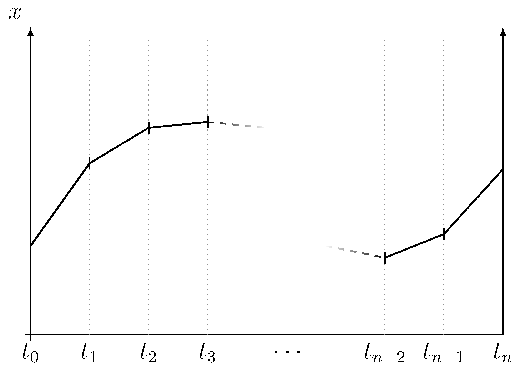
\includegraphics[scale=1.0]{../figures/illustrations/lqcd/path-integral/path-integral-flattened}
\end{figure}}
\only<2->{\begin{align*}
    \langle O \rangle = \mathcolor{red}{\frac{1}{Z}\int\mathcal{D}U} O[U] \mathcolor{red}{\e^{- S_G[U]}}.
\end{align*}
with 
\begin{align*}
Z = \int \mathcal{D}U e^{- S_G[U]}.
\end{align*}}
\onslide <3->{We will use the \textit{Metropolis algorithm} to create configurations of the lattice.}
\note{
    \begin{itemize}
        \item<1->{An example of the discretized path integral, going from time $t_0$ to $t_{n}$, where the end points is taken to be equal, $x_0=x_{N_T}$. We integrate over all of space at each time $t_i$ finding the most likely position at a given time.}
        \item<2->{We will use the parts marked in red as a probability distribution which we will create configurations from.}
        \item<3->{This can be used in the \textit{Metropolis algorithm.}}
        \item<4->{Since a path integral integrates over all possible configurations, our job us to generate enough configurations to properly represent the statistics.}
    \end{itemize}
}
\end{frame}

\begin{frame}{Measurements on the lattice}
The observable becomes an average over the $N_\mathrm{MC}$ gauge configurations.
\begin{align*}
    \expect{O} = \underset{N_\mathrm{MC}\rightarrow\infty}{\lim} \frac{1}{N_\mathrm{MC}} \sum^{N_\mathrm{MC}}_i O[U_i]
\end{align*}
\onslide<1->We now need to generate configurations...
\note{
\begin{itemize}
    \item We perform an average of the created configurations.
\end{itemize}
}
\end{frame}

% \begin{frame}{The Metropolis algorithm}
% \begin{algorithmic}
%     \Repeat
%         \State Randomly generate a candidate state $j$ with probability $T_{i\rightarrow i}$.
%         \State Calculate $A_{i\rightarrow j}$ which saw on previous slide.
%         \State Generate random number $u\in[0,1]$.
%         \If {$u \leq A_{i\rightarrow j}$}
%             \State Accept new state $j$.
%         \ElsIf {$u > A_{i\rightarrow j}$}
%             \State Reject new state $j$ and retain the old state $i$.
%         \EndIf
%     \Until {$N_\mathrm{MC}$ samples are generated.}
% \end{algorithmic}
% \note{
% \begin{itemize}
%     \item Generated state $j$ is a gauge configuration.
%     \item Algorithm of choice when sampling gauge configurations.
%     \item For generating $N_\mathrm{MC}$ Monte Carlo samples.
% \end{itemize}
% }
% \end{frame}

% \begin{frame}{The Metropolis algorithm on the lattice}
% A parameter $\epsilon_\mathrm{rnd}$ controls the spread of the candidate matrices.
% \begin{enumerate}
%     \item Initialize lattice with $\SU(3)$ matrices close to unity(\textit{hot start}) or at unity(\textit{cold start}).
%     \item Thermalize with $N_\mathrm{therm}$ sweeps.
%     \item Generate $N_\mathrm{MC}$ samples,
%     \begin{enumerate}[i]
%         \item Perform $N_\mathrm{corr}$ correlation updates.
%         \item At each update, perform $N_\mathrm{up}$ single link update for every lattice link.
%         \item Store configuration and/or apply gradient flow and sample observables on it.
%     \end{enumerate}
% \end{enumerate}
% \note{
% \begin{itemize}
%     \item We use \textbf{periodic boundary conditions} for all calculations.
%     \item $N_\mathrm{MC}$ is how many configurations we will generate.
%     \item $N_\mathrm{up}$ is how many single link updates we will perform.
%     \item $N_\mathrm{corr}$ is how many full sweeps we shall perform in between each sampling. Needed in order to reduce the autocorrelation between the configurations.
%     \item We checked that our choice for the matrix generation parameter $\epsilon_\mathrm{rnd}$ minimizes the autocorrelation.
% \end{itemize}
% }
% \end{frame}

\begin{frame}{Parallelization}
\onslide<1->{The lattice now is a 4D hypercube, with four links associated to each lattice site \rightarrow need to parallelize!


}%
\onslide<2->{Two methods used:}
\begin{itemize}
    \item<3->{ Single link sharing used in the Metropolis algorithm.}
    \item<4->{ \textit{shifts} used in in gradient flow and observable sampling}
\end{itemize}
\note{
\begin{itemize}[<+->]
    \item Due to the size of the lattice, we need to parallelize!.
    \item We parallelized using \textbf{MPI}.
    \item Tested out \textbf{halos}, but turned out to be problematic when generating.
\end{itemize}
}
\end{frame}

\begin{frame}{Shifts}
\begin{figure}
    \centering
    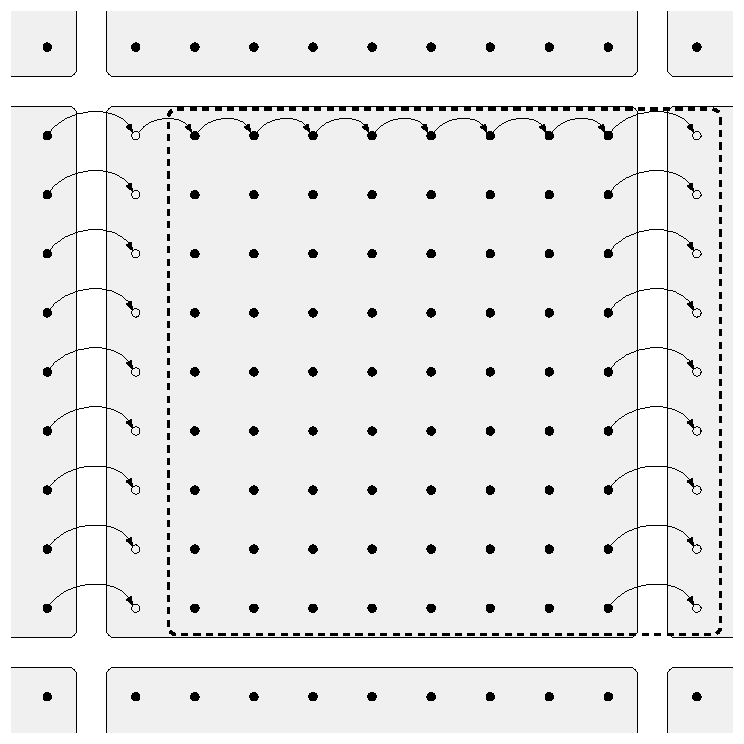
\includegraphics[scale=0.6]{../figures/illustrations/implementation/shift/shift}
\end{figure}
\note{
\begin{itemize}
    \item An illustration of the lattice shift. 
    \item The links $U_\nu$ of the lattice are copied over to a temporary lattice shifted in direction $\hat{\mu}$. 
    \item The face that is shifted over to an adjacent sub-lattice is shared through a non-blocking MPI call, while we copy the links to the temporary lattice.
    \item Allows for a simplified syntax close to that of the equations we are working with.
    \item Don't have to write out any loops over the lattice positions.
\end{itemize}
}
\end{frame}

%%%%%%%%%%%%%%%%%%%%%%%%%%%%%%%%%%%%%%%%%%%%%%%%%%%%%%%%%%%%%%%%%%%%%%%%%%%%%%%%%%%%%%%%%%
%   ____               _ _            _      __ _
%  / ___|_ __ __ _  __| (_) ___ _ __ | |_   / _| | _____      __
% | |  _| '__/ _` |/ _` | |/ _ \ '_ \| __| | |_| |/ _ \ \ /\ / /
% | |_| | | | (_| | (_| | |  __/ | | | |_  |  _| | (_) \ V  V /
%  \____|_|  \__,_|\__,_|_|\___|_| |_|\__| |_| |_|\___/ \_/\_/
%%%%%%%%%%%%%%%%%%%%%%%%%%%%%%%%%%%%%%%%%%%%%%%%%%%%%%%%%%%%%%%%%%%%%%%%%%%%%%%%%%%%%%%%%%
\section{Gradient flow}
\husk{TODO: ANIMATIONS?!}
\begin{frame}{The flow equation}
% Bad approx.: diffusion equation
% Topological charge preserved and is more pronounced 
% Why it is needed
% Certain quantities becomes renormalizable
The flow of the $\SU(3)$ gauge fields are denoted by $B_\mu(x,t_f)$ which are Lie algebra valued gauge fields,
\onslide<1->{\begin{align*}
    \frac{\dd}{\dd t_f} B_\mu(x,t_f) = D_\nu G_{\nu\,\mu}(x,t_f), \label{eq:flow-continuum-diff-eq}
\end{align*}}
\onslide<2->{\begin{align*}
    D_\mu = \partial_\mu + \left[B_\mu(x,t_f), \cdot \right], \label{eq:flow-cont-covariant-derivative}
\end{align*}}
\onslide<3->{\begin{align*}
    G_{\mu\nu}(x,t_f) = \partial_\mu B_\nu(x,t_f) - \partial_\nu B_\mu(x,t_f) - i[B_\mu(x,t_f), B_\nu(x,t_f)], \label{eq:flow-field-strength-tensor}
\end{align*}}
\onslide<4->{with the initial conditions being the fundamental gauge field,
\begin{align*}
    B_\mu(x,t_f)|_{t_f=0} = A_\mu(x).
\end{align*}}
\onslide<5->{
A bad approximation: \textit{the diffusion equation}, 
\begin{align*}
    \frac{\partial}{\partial t_f} B_\mu(x,t_f) \approx \partial^2 B_\mu(x,t_f)
\end{align*}
}
\onslide<6->{
    The smearing radius increases as $\sqrt{8t_f}$.
}
\note{
\begin{itemize}
    \item <1->The flow equation in the continuum is defined by this differential equation.
    \item <2->With the covariant derivative given by following, with the $\cdot$ being the derivative with respect to flow time.
    \item <3->The field strength tensor of the flown fields is given in the regular format.
    \item <4->The initial condition is the un-flowed gauge field, $A_\mu$.
    \item <5->Bad approx.: diffusion equation.
    \item <6->Topological charge preserved and is more pronounced.
    \item <6->Renormalizes the topological charge at non-zero flow time.
\end{itemize}
}
\end{frame}

\begin{frame}{Gradient flow on the lattice}
% RK3 classical and then on the lattice
\onslide<1->{Lattice definition given by
\begin{align*}
    \dot{V}_{t_f}(x,\mu) = - g_S^2 \left\{\partial_{x,\mu} S_G[V_{t_f}] \right\} V_{t_f}(x,\mu),
\end{align*}}
\onslide<2->{with initial condition,
\begin{align*}
    V_{t_f}(x,\mu)|_{t_f=0} = U(x,\mu)
\end{align*}}
\onslide<3->{Note: need to find the action derivative $S_G[V_{t_f}]$.}
\note{
\begin{itemize}
    \item <1->On the lattice, the flow equation takes the shape in terms of the link variables.
    \item <2->Initial conditions similar to the continuum case.
    \item <3->The action derivative is also needed, but that is a minor task we will not cover here.
\end{itemize}
}
\end{frame}

\begin{frame}{Solving gradient flow with Runge-Kutta 3}
\onslide<1->{With
\begin{align*}
    \dot{V}_{t_f} = - g_S^2 \left\{\partial_{x,\mu} S_G[V_{t_f}] \right\} V_{t_f} = Z(V_{t_f}) V_{t_f},
\end{align*}}
\onslide<2->{and $Z_i=\epsilon_fZ(W_i)$ we get
\begin{align*}
    \begin{split}
        &W_0 = V_{t_f}, \\
        &W_1 = \exp\left[\frac{1}{4}Z_0\right]W_0, \\
        &W_2 = \exp\left[\frac{8}{9}Z_1 - \frac{17}{36}Z_0\right]W_1, \\
        &V_{t_f + \epsilon_f} = \exp\left[\frac{3}{4}Z_2 - \frac{8}{9}Z_1 + \frac{17}{36}Z_0\right]W_2, \\
    \end{split}
\end{align*}
with coefficients from \citet{luscher_properties_2010}.}
\note{
\begin{itemize}
    \item <1->{ We rewrite the equations slightly,}
    \item <2->{ and use a structure preserving integrator with coefficients from \citet{luscher_properties_2010}.}
    \item <3->{ We control the accuracy of this integrator by $\epsilon_f$.}
\end{itemize}}
\end{frame}

\husk{TODO: animation here!!}

\begin{frame}{Verifying the integration} \husk{TODO: REMOVE THIS?!?!}
\only<1>{Testing the integrator for different integration steps $\epsilon_f$.
\begin{table}
    \centering
    \resizebox{0.8\columnwidth}{!}{%
    \begin{tabular}{c c c c c c c c c c c}
    \toprule
    $\epsilon_f$ & $0.001$ & $0.005$ & $0.007$ & $0.009$ & $0.01$ & $0.02$ & $0.03$ & $0.05$ & $0.1$ & $0.5$ \\ \bottomrule
    \end{tabular}
    }
\end{table}}
\only<2>{Lattice size $N^3\times N_T = 24^3 \times 48$ with $\beta=6.0$.
\vspace{-10.0pt}
\begin{figure}
    \centering
    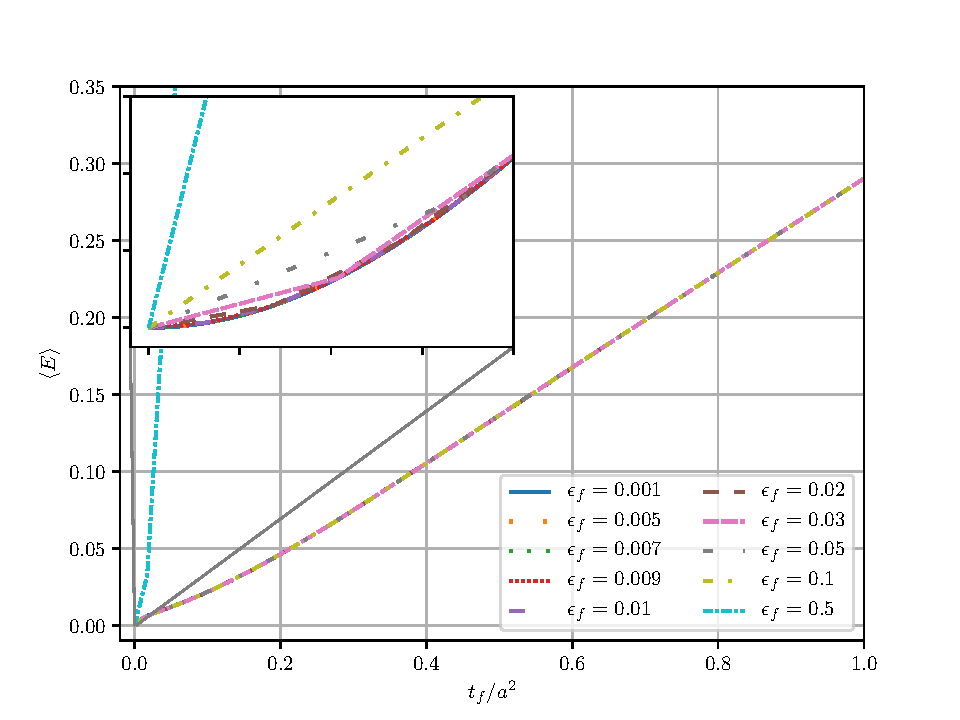
\includegraphics[trim={0.4cm 0.0cm 0.4cm 0.0cm},clip,scale=0.6]{../figures/flow-epsilon/energy}
\end{figure}}
\only<3->{The absolute difference between the smallest flow time $\epsilon_f=0.001$ and those shown previously.
\vspace{-10.0pt}
\begin{figure}
    \centering
    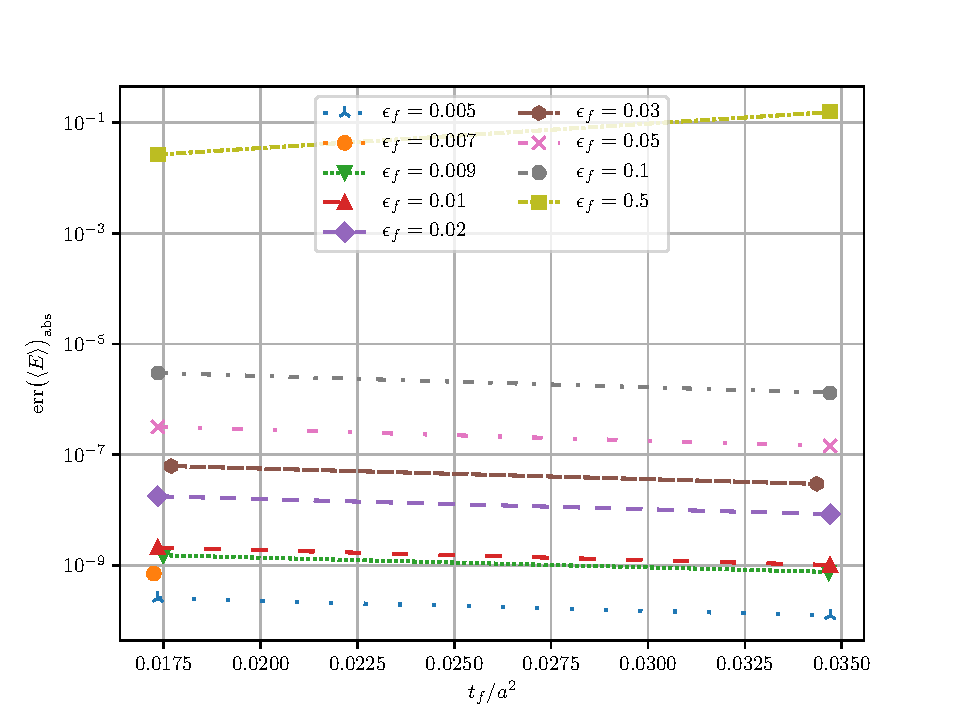
\includegraphics[trim={0.4cm 0.0cm 0.4cm 0.0cm},clip,scale=0.6]{../figures/flow-epsilon/energy_diff_absolute}
\end{figure}}
\note{
\begin{itemize}
    \item<1-> The values we will test the integrator against.
    \item<2-> The energy flowed for different the different $\epsilon_f$ values.
    \item<3-> The absolute difference between the smallest flow time $\epsilon_f=0.001$ and those listed in previous table.
    \item<3-> The reason for \textbf{only having two points} is due to the fact that we are only \textbf{comparing points} that are \textbf{close to each other in flow time}. If we were to have more points, we would have to double the number of flow time steps for the smallest lattices.
    \item<4-> An \textbf{example} of the flowing, can be seen by observing the \textbf{energy evolving over flow time}.
\end{itemize}}
\end{frame}

% \begin{frame}{Smearing the lattice: topological charge I}
% \begin{center}
%     \animategraphics[loop,controls,width=\linewidth,scale=0.6]{15}{../figures/latviz/topc_TE21/flowTime_TE21-}{0}{60}
% \end{center}
% \note{
% \begin{itemize}
%     \item Me and Giovanni Pederiva created a program for visualizing the gauge field.
%     \item Shows how the flow "removes noise" from the lattice, and only leaves large scale structures intact.
% \end{itemize}}
% \end{frame}

% \begin{frame}{Smearing the lattice: topological charge II}
% \begin{center}
%     \animategraphics[loop,controls,width=\linewidth,scale=0.7]{15}{../figures/latviz/topc_TE27/flowTime_TE27-}{0}{60}
% \end{center}
% \end{frame}

% \begin{frame}{Smearing the lattice: topological charge III}
% \begin{center}
%     \animategraphics[loop,controls,width=\linewidth,scale=0.7]{15}{../figures/latviz/topc_TF500/euclideanTime_tf500--}{0}{63}
% \end{center}
% \end{frame}


%%%%%%%%%%%%%%%%%%%%%%%%%%%%%%%%%%%%%%%%%%%%%%%%%%%%%%%%%%%%%%%%%%%%%%%%%%%%%%%%%%%%%%%%%%
%  ____                 _ _
% |  _ \ ___  ___ _   _| | |_ ___
% | |_) / _ \/ __| | | | | __/ __|
% |  _ <  __/\__ \ |_| | | |_\__ \
% |_| \_\___||___/\__,_|_|\__|___/
%%%%%%%%%%%%%%%%%%%%%%%%%%%%%%%%%%%%%%%%%%%%%%%%%%%%%%%%%%%%%%%%%%%%%%%%%%%%%%%%%%%%%%%%%%
\section{Results}

\begin{frame}{Ensembles}
% Include size and time
\begin{table}
    \centering
    \begin{tabular}{l r r r r r r}
        \toprule
        Ensemble & $\beta$ & $N$ & $N_T$ & $N_\mathrm{cfg}$ & $\epsilon_\mathrm{flow}$ & Config. size$[$GB$]$ \\ 
        \midrule
        $A$   & 6.0  & 24 & 48 & 1000 & 0.01 & 0.356 \\
        $B$   & 6.1  & 28 & 56 & 1000 & 0.01 & 0.659 \\
        $C$   & 6.2  & 32 & 64 & 2000 & 0.01 & 1.125 \\
        $D_1$ & 6.45 & 32 & 32 & 1000 & 0.02 & 0.563 \\
        $D_2$ & 6.45 & 48 & 96 & 250  & 0.02 & 5.695 \\
        \bottomrule
    \end{tabular}
\end{table}
\husk{TODO: Remove bit about updating frequency?}
\begin{itemize}[<+->]
    \item We use $N_\mathrm{corr}=1600$ for $\beta=6.45$ ensembles, $N_\mathrm{corr}=600$ for the rest.
    \item $N_\mathrm{up}=30$.
\end{itemize}
\note{
\begin{itemize}
    \item The main ensembles made for this thesis. 
    \item Every configuration was flown with $N_\mathrm{flow}=1000$ flow steps.
    \item We should also mention that we generated a few additional ensembles for investigating other aspects of the topological charge.
\end{itemize}
}
\end{frame}

\begin{frame}{Lattice sizes}
\begin{table}
    \centering
    \begin{tabular}{l r r r}
        \toprule
        Ensemble     & $L/a$           & $L$ $[\fm]$     & $a$ $[\fm]$     \\ \midrule
        $A$          & $24$            & $2.235(9)$      & $0.0931(4)$     \\ 
        $B$          & $28$            & $2.214(10)$     & $0.0791(3)$     \\ 
        $C$          & $32$            & $2.17(1)$       & $0.0679(3)$     \\ 
        $D_1$        & $32$            & $1.530(9)$      & $0.0478(3)$     \\ 
        $D_2$        & $48$            & $2.29(1)$       & $0.0478(3)$     \\ 
        \bottomrule
    \end{tabular}
\end{table}
Charge radius of a proton: $\sim 0.85$ fm.
\note{The lattice sizes.}
\end{frame}


\begin{frame}{Energy definition}
\onslide<1->{\begin{align*}
    E &= \frac{a^4}{2|\Lambda|} \sum_{n\in\Lambda}\sum_{\mu,\nu} \left(F^\mathrm{clov}_{\mu\nu}(n)\right)^2 \\
\end{align*}}
\onslide<2->{We can use this definition to set a scale $t_0$,
\begin{align*}
    \left\{t^2_f \expect{E(t)} \right\}_{t_f = t_{0}} = 0.3.
\end{align*}
}
\note{
\begin{itemize}
    \item Defined as the field strength tensor squared averaged over all lattice points and directions.
    \item We can use this definition to set a scale.
\end{itemize}
}
\end{frame}

\begin{frame}{The clover field strength definition}
$F_{\mu \nu}^\mathrm{clov}(n)$ is given by
\begin{figure}
    \centering
    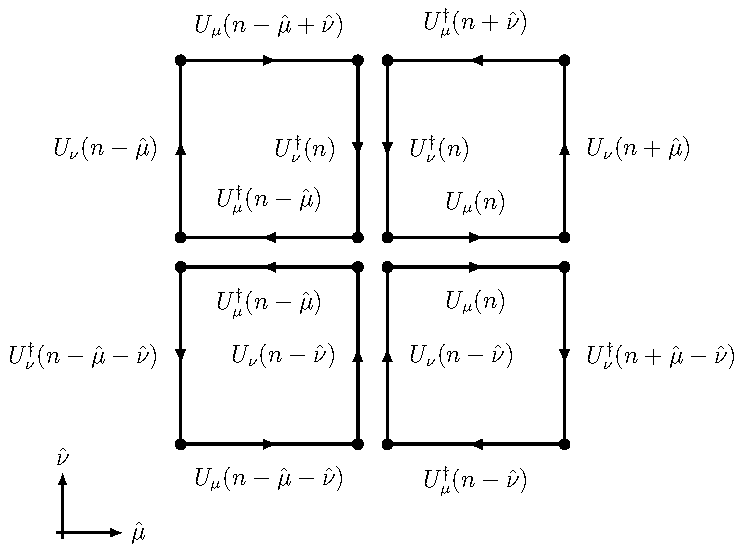
\includegraphics[scale=0.7]{../figures/illustrations/lqcd/clover/clover}
\end{figure}
\note{
\begin{itemize}
    \item We will use the clover field strength definition in gauge observables.
    \item \textbf{Symmetries} will allow us to \textbf{reduce} the effective \textbf{number of clovers} need to \textbf{calculate from 24 to 6}.
\end{itemize}
}
\end{frame}

\begin{frame}{Energy}
\vspace{-10.0pt}
\begin{figure}
    \centering
    \includegraphics[trim={0.2cm 0.0cm 0.2cm 0.5cm},clip,scale=0.7]{../../LQCD/LatticeAnalyser/figures_b645_32xx4_full/data11/post_analysis/energy/post_analysis_energy_bootstrap_zoomed.pdf}
\end{figure}
\end{frame}

% \begin{frame}{Scale setting \texorpdfstring{$t_0$}{t0}}
% \only<1>{\begin{table}
%     \centering
%     \begin{tabular}{l r r r}
%         \toprule
%         Ensemble     & $L/a$           & $L$ $[\fm]$     & $a$ $[\fm]$     \\ \midrule
%         $A$          & $24$            & $2.235(9)$      & $0.0931(4)$     \\ 
%         $B$          & $28$            & $2.214(10)$     & $0.0791(3)$     \\ 
%         $C$          & $32$            & $2.17(1)$       & $0.0679(3)$     \\ 
%         $D_1$        & $32$            & $1.530(9)$      & $0.0478(3)$     \\ 
%         $D_2$        & $48$            & $2.29(1)$       & $0.0478(3)$     \\ 
%         \bottomrule
%     \end{tabular}
% \end{table}
% }
% \only<2->{\begin{table} % Not needed since I present the continuum extrapolation in the next figure.
%     \centering
%     \begin{tabular}{l r r r}
%         \toprule
%         Ensemble     & $t_0$[fm$^2$]   & $t_0/a^2$       & $t_0/r_0^2$     \\ \midrule
%         $A$          & $0.02780(2)$    & $3.20(3)$       & $0.11121(9)$    \\ 
%         $B$          & $0.02769(2)$    & $4.43(4)$       & $0.11075(10)$   \\ 
%         $C$          & $0.02775(2)$    & $6.01(6)$       & $0.11099(8)$    \\ 
%         $D_1$        & $0.02779(5)$    & $12.2(1)$       & $0.1112(2)$     \\ 
%         $D_2$        & $0.02794(9)$    & $12.2(1)$       & $0.1117(3)$     \\ 
%         \bottomrule
%     \end{tabular}
% \end{table}}
% \note{
% \begin{itemize}
%     \item <2->Extrapolation results for $t_0$, where we retrieved the exact point of intersection between $t_f^2 \expect{E}$ and $0.3$ using $N_\mathrm{bs}=500$ bootstrap fits. Extrapolating to the continuum gives us $t_{0,\mathrm{cont}}/r_0^2 = 0.11087(50)$.
% \end{itemize}
% }
% \end{frame}

\begin{frame}{Scale setting \texorpdfstring{$t_0$}{t0}}
\onslide<1->{
\vspace{-5.0pt}
\begin{figure}
    \centering
    \includegraphics[trim={0.2cm 0.25cm 0.2cm 1.2cm},clip,scale=0.6]{../../LQCD/LatticeAnalyser/figures/data11/post_analysis/energy/post_analysis_extrapmethodbootstrap_t0reference_continuum_bootstrap.pdf}
\end{figure}
}
\onslide<2->{\vspace{-5.0pt}Continuum extrapolation using ensembles $A$, $B$, $C$, and $D_2$ gives $t_{0,\mathrm{cont}}/r_0^2 = 0.11087(50)$.}
\onslide<3->{This matches the values retrieved by \citet{luscher_properties_2010}.}
\note{
\begin{itemize}
    \item <1->The continuum extrapolation $a\rightarrow 0$ for $t_0$ of the four ensembles $A$, $B$, $C$, and $D_2$.
    \item <2->$r_0=0.5$ fm.
\end{itemize}
}
\end{frame}

\begin{frame}{Scale setting \texorpdfstring{$t_0$}{t0}}
\onslide<1->{Extrapolations for different ensemble-combinations
\begin{table}
    \centering
    \begin{tabular}{l r r}
        \toprule
        Ensembles               & $t_{0,\mathrm{cont}}/r_0^2$   & $\chi^2/\mathrm{d.o.f}$ \\ \midrule
        $A$, $B$, $C$, $D_2$    & $0.11087(50)$                         & $7.51$ \\
        $B$, $C$, $D_2$         & $0.1115(3)$                           & $0.41$ \\
        $A$, $B$, $C$, $D_1$    & $0.1119(6)$                           & $0.88$ \\
        \bottomrule
    \end{tabular}
\end{table}}
\note{
    \begin{itemize}
        \item Notice the $\chi^2/\text{d.o.f.}$ of the extrapolation versus the two other extrapolations.
    \end{itemize}
}
\end{frame}

\begin{frame}{Scale setting \texorpdfstring{$w_0$}{w0}}
\only<1>{Can also set a scale using the derivative which offers more granularity for small flow times,
\begin{align*}
    &W(t)|_{t=w_0^2} = 0.3, \\
    &W(t) \equiv t_f \frac{\dd}{\dd t_f} \left\{t^2_f \expect{E}\right\}.
\end{align*}
First presented by \citet{borsanyi_high-precision_2012}.
}
\onslide<2->{\begin{table}
    \centering
    \begin{tabular}{l r r}
        \toprule
        Ensembles               & $w_{0,\mathrm{cont}}$[fm]  & $\chi^2/\mathrm{d.o.f}$ \\ \midrule
        $A$, $B$, $C$, $D_2$    & $0.1695(5)$               & $7.12$ \\
        $B$, $C$, $D_2$         & $0.1702(3)$               & $0.53$ \\
        $A$, $B$, $C$, $D_1$    & $0.1706(6)$               & $0.86$ \\
        \bottomrule
    \end{tabular}
\end{table}}
\onslide<3->{Comparable to \citet{borsanyi_high-precision_2012} which included dynamical fermions, with $w_{0,\mathrm{cont}}=0.1755(18)(04)$ fm.}
\end{frame}

% \begin{frame}{HERE}
% <<<<<<<<<<<<<<<<<<<<<<<<<<<<<<<<<<<<<<<<<<<<<<<<<<<<<<<<<<<<<<<<<<<<<<<<<<<<<<<<<<<<<<<<<<<<<<<<<<<<<<
% <<<<<<<<<<<<<<<<<<<<<<<<<<<<<<<<<<<<<<<<<<<<<<<<<<<<<<<<<<<<<<<<<<<<<<<<<<<<<<<<<<<<<<<<<<<<<<<<<<<<<<
% <<<<<<<<<<<<<<<<<<<<<<<<<<<<<<<<<<<<<<<<< YOU ARE HERE <<<<<<<<<<<<<<<<<<<<<<<<<<<<<<<<<<<<<<<<<<<<<<<
% <<<<<<<<<<<<<<<<<<<<<<<<<<<<<<<<<<<<<<<<<<<<<<<<<<<<<<<<<<<<<<<<<<<<<<<<<<<<<<<<<<<<<<<<<<<<<<<<<<<<<<
% <<<<<<<<<<<<<<<<<<<<<<<<<<<<<<<<<<<<<<<<<<<<<<<<<<<<<<<<<<<<<<<<<<<<<<<<<<<<<<<<<<<<<<<<<<<<<<<<<<<<<<
% \end{frame}


\begin{frame}{Topological charge}
\begin{block}{}
\begin{itemize}
    \item <1->{Gauge fields can be classified by their topological properties.}
    \item <2->{\textbf{Topological charge} $Q$ can be viewed as a ``measure'' of instantons.}
    \item <3->{\textbf{Instantons} are local minimums of the Yang-Mills action in Euclidean space.}
\end{itemize}
\end{block}
% \only<1>{\begin{figure}
%     \centering
%     \begin{subfigure}{0.22\textwidth}
%         \centering
%         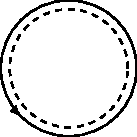
\includegraphics{../figures/illustrations/qcd/winding-number/winding-number1.pdf}
%         \caption{$\nu=+1$}
%     \end{subfigure}
%     \begin{subfigure}{0.22\textwidth}
%         \centering
%         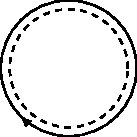
\includegraphics{../figures/illustrations/qcd/winding-number/winding-number-1.pdf}
%         \caption{$\nu=-1$}
%     \end{subfigure}
%     \begin{subfigure}{0.22\textwidth}
%         \centering
%         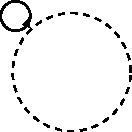
\includegraphics{../figures/illustrations/qcd/winding-number/winding-number0.pdf}
%         \caption{$\nu=0$}
%     \end{subfigure}
%     \begin{subfigure}{0.22\textwidth}
%         \centering
%         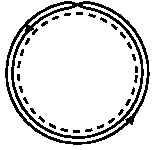
\includegraphics{../figures/illustrations/qcd/winding-number/winding-number+2.pdf}
%         \caption{$\nu=+2$}
%     \end{subfigure}
%     \caption{The figure is taken from \citet[p. 32]{forkel_primer_2000}.}
% \end{figure}}
\onslide<4->{
    \begin{align*}
        Q = a^4 \sum_{n\in\Lambda} q(n),
    \end{align*}
    with the charge density given by
    \begin{align*}
        q(n) = \frac{1}{32\pi^2} \epsilon_{\mu\nu\rho\sigma} \tr\left[F_{\mu\nu}(n)F_{\rho\sigma}(n)\right].
    \end{align*}
}
\onslide<5->{
\begin{align*}
    \expect{Q} = 0
\end{align*}
}
\note{
% Now we are going to look at another important quantity in pure gauge lattice theory, namely topological charge. In order to appreciate the results, let me first introduce what is meant by topological charge.
\begin{itemize}
    % \item <1->An illustration of how one can view the winding number given a function $f$ that parametrizes a path around a circle $S^1$. Given that it starts and ends at the same point, we have that the number of times it wraps around the circle gives us the winding number.
    \item <2->Measuring \textbf{topological charge} is a measure of the \textit{Winding number} of the gauge field.
    \item <3->\textbf{Instantons} are local minimums to the Yang-Mills action in Euclidean space.
    \item <3->Instantons are significant in LQCD because of \textit{critical slowdown} which we will return to later.
    \item <4->The charge is a \textbf{sum over the local charge} at every point in the gauge field. 
    \item <4->Can in a very crude manner be viewed as the ``curl'' of the gauge fields.
    \item <5->The \textbf{expectation value} of \textbf{$Q$ is zero} due to it being \textbf{parity odd}.
\end{itemize}
}
\end{frame}

% \begin{frame}{Topological charge}
% We will use the \textit{clover field strength definition} instead of the plaquette for the field strength.
% \begin{figure}
%     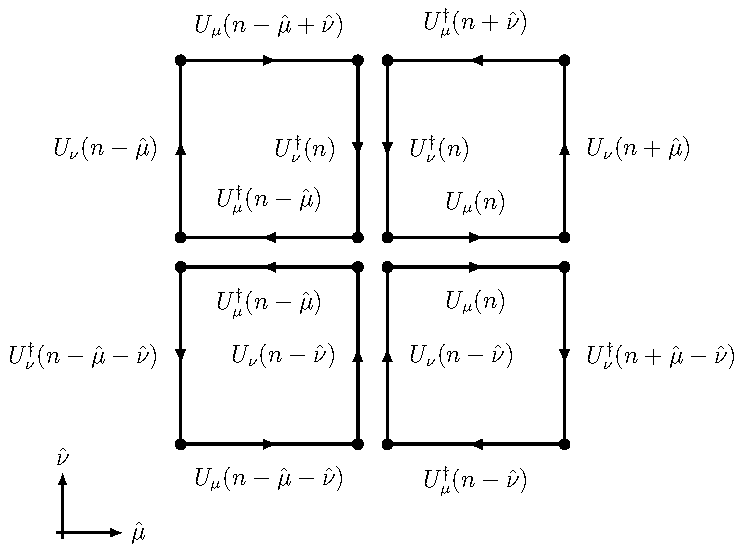
\includegraphics[scale=0.7]{../figures/illustrations/lqcd/clover/clover.pdf}
% \end{figure}
% \note{
% \begin{itemize}
%     \item We will use the clover field strength definition.
%     \item Symmetries will allow us to reduce the effective number of clovers need to calculate from 24 to 6.
% \end{itemize}
% }
% \end{frame}

\husk{TODO: topological charge animation here!!}

\begin{frame}{Topological charge distribution}
\vspace{-5.0pt}
\begin{figure}
    \centering
    \includegraphics[trim={0.2cm 0.0cm 0.2cm 1.0cm},clip,scale=0.7]{../../LQCD/LatticeAnalyser/figures/beta61_16x32_run/topc/topc_multihistogram_beta6_1}
\end{figure}
\note{Histograms for the $Q$ for ensemble $G$ with a lattice of size $N^3\times N_T=16^3\times 32$ with $\beta=6.1$, taken at different flow times $t_f/a^2=0.0$, $1.0$, $4.0$ fm.}
\end{frame}

\begin{frame}{Topological charge distribution in flow time}
\vspace{-5.0pt}
\begin{figure}
    \centering
    \includegraphics[trim={0.2cm 0.0cm 0.2cm 1.0cm},clip,scale=0.7]{../../LQCD/LatticeAnalyser/figures/topc_modes_analysis/topc_modes_tf250.pdf}
\end{figure}
\note{Histograms of topological charge for the supporting ensembles seen at $t_f/a^2=0.25$ fm.}
\end{frame}


\begin{frame}{Topological charge for our main ensembles}
\vspace{-5.0pt} 
\begin{figure}
    \centering
    \includegraphics[trim={0.2cm 0.0cm 0.2cm 1.0cm},clip,scale=0.7]{../../LQCD/LatticeAnalyser/figures_b645_32xx4_full/data11/post_analysis/topc/post_analysis_topc_bootstrap.pdf}
\end{figure}
\note{\begin{itemize}[<+->]
    \item Topological charge $Q$ as evolved in flow time for the five main ensembles.
    \item The ensemble $D_1$ is okay to include, as the topological charge becomes independent of the volume around a side length of $\sim 1.2$-$1.3$ fermi.
    \item Bootstrapped data with $N_\mathrm{bs}=500$ bootstrap samples.
    \item Corrected for autocorrelations with $\sigma = \sqrt{2 \tau_\mathrm{int}} \sigma_0$.
\end{itemize}
}
\end{frame}

\begin{frame}
\vspace{5.0pt}
\begin{center}
Why is the charge not centered around zero for certain ensembles?
\end{center}
\end{frame}

\begin{frame}{Autocorrelation in the energy}
\begin{figure}
    \centering
    \includegraphics[trim={0.2cm 0.0cm 0.2cm 1.0cm},clip,scale=0.6]{../../LQCD/LatticeAnalyser/figures_b645_32xx4_full/data11/post_analysis/energy/post_analysis_energy_bootstrap_autocorr.pdf}
\end{figure}
\note{The autocorrelation of the energy. A value of $\tau_\mathrm{int}=0.5$ indicates that we have zero autocorrelation.}
\end{frame}

\begin{frame}{Topological charge autocorrelation}
\vspace{-5.0pt}
\begin{figure}
    \centering
    \includegraphics[trim={0.2cm 0.0cm 0.2cm 1.0cm},clip,scale=0.7]{../../LQCD/LatticeAnalyser/figures_b645_32xx4_full/data11/post_analysis/topc/post_analysis_topc_bootstrap_autocorr.pdf}
\end{figure}
\note{
\begin{itemize}
    \item The integrated autocorrelation $\tau_\mathrm{int}$ for topological charge for the five main ensembles.
\end{itemize}
}
\end{frame}

% \begin{frame}{Additional ensembles}
% \begin{table}
%     \centering
%     \resizebox{0.8\columnwidth}{!}{%
%     \begin{tabular}{l r r r r r r r}
%         \toprule
%         Ensemble & $N$ & $N_T$ & $N_\mathrm{cfg}$ & $N_\mathrm{corr}$ & $N_\mathrm{up}$ & $a$ $[\fm]$ & $L$ $[\fm]$ \\ 
%         \midrule
%         $E$ & 8 & 16 & 8135 & 600 & 30 & 0.0931(4) & 0.745(3) \\
%         $F$ & 12 & 24 & 1341 & 200 & 20 & 0.0931(4) & 1.118(5) \\
%         $G$ & 16 & 32 & 2000 & 400 & 20 & 0.0790(3) & 1.265(6) \\
%         \bottomrule
%     \end{tabular}
%     }
% \end{table}
% \note{\begin{itemize}
%     \item Additional ensembles made in order to illuminate additional aspects of the topological charge.
%     \item Supporting ensembles made on Smaug. All ensembles were flown $N_\mathrm{flow}=1000$ steps with $\epsilon_\mathrm{flow}=0.01$.
% \end{itemize}}
% \end{frame}

\begin{frame}{Critical slowdown}
\onslide<1->{\textbf{Critical slowdown} is the phenomena where we as the lattice spacing $a$ \textit{decreases} the required energy to tunnel from one state to another \textit{increase}. \\}
\onslide<2->{$\rightarrow$ many more lattice updates are required in order to have independent gauge configurations.}
\note{
\begin{itemize}
    \item <2->That is, going from one instanton sector to another requires many more updates and becomes an inherent problem in all LQCD calculations.
    \item <3->In the continuum it would require an \textbf{infinite amount of energy} to go from \textbf{one instanton sector to another}. Thus as we \textbf{$a$ approaches the continuum}, the amount of \textbf{effort}(number of updates ect.) required to generate \textbf{independent} gauge configurations \textbf{increases}.
\end{itemize}}
\end{frame}

\begin{frame}{Topological susceptibility}
\husk{TODO: WHat is hadronic scales again?}
\onslide<1->{
The \textit{topological susceptibility} is given by
\begin{align*}
    \chi_\mathrm{top}^{1/4} = \frac{1}{V^{1/4}}\expect{Q^2}^{1/4}
\end{align*}
with $V$ being the lattice volume and $\expect{Q^2}$ is the second momenta of the charge. \\}
\onslide<2->{
The \textit{Witten-Veneziano relation} is given by \husk{TODO: rearrange!?!}
\begin{align*}
    m_{\eta'}^2 = \frac{2N_f}{f^2_\pi}\chi_\mathrm{top}
\end{align*}}
\onslide<3->{with}
\begin{block}{}
\begin{itemize}
    \item <3->pion decay constant $f_\pi=0.130(5)/\sqrt{2}$ GeV.
    \item <4->$\eta'$ meson mass $m_{\eta'}=0.95778(6)$ GeV.
    \item <5->$N_f$ is the number of flavors(i.e. quark species involved in $\eta'$.).
\end{itemize}
\end{block}
\onslide<6->{We expect $N_f=3$.}
\note{
\begin{itemize}
    \item <2->R.h.s. is full QCD and l.h.s is from pure gauge theory.
    \item <3->We can use the Witten-Veneziano formula in order to extract an estimate for $N_f$ using the topological susceptibility.
    \item <6->This can help us understand the "quality" of the ensemble, as we would expect to be around $N_f=3$.
\end{itemize}
}
\end{frame}

\begin{frame}{Topological susceptibility}
\begin{figure}
    \centering
    \includegraphics[trim={0.2cm 0.0cm 0.2cm 1.0cm},clip,scale=0.7]{../../LQCD/LatticeAnalyser/figures_b645_32xx4_full/data11/post_analysis/topsus/post_analysis_topsus_bootstrap.pdf}
\end{figure}
\note{\begin{itemize}
    \item The topological susceptibility $\chi^{1/4}_{t_f}$ of the \textbf{main ensembles}.
    \item We have a \textbf{UV divergence at zeroth flow time}, hence to need for gradient flow which renormalizes this quantity.
    \item \textbf{Bootstrapped} $N_\mathrm{bs}=500$ times.
    \item \textbf{Corrected for autocorrelations} with $\sigma = \sqrt{2 \tau_\mathrm{int}} \sigma_0$.
\end{itemize}}
\end{frame}

\begin{frame}{Topological susceptibility continuum extrapolation}
\begin{table}
    \centering
    \begin{tabular}{l r r r}
        \toprule
        Ensemble     & $\chi_{t_f}^{1/4}$ [GeV] & $\chi_{t_f}^{1/4}$ [GeV], corrected & $\sqrt{2\tau_\mathrm{int}}$\\
        \midrule
        $A$          & $0.1877(23)$ & $0.1877(24)$  & $1.028(46)$  \\
        $B$          & $0.1880(21)$ & $0.1880(29)$  & $1.346(81)$  \\
        $C$          & $0.1853(14)$ & $0.1853(24)$  & $1.762(104)$ \\
        $D_1$        & $0.1971(22)$ & $0.1971(101)$ & $4.523(675)$ \\
        $D_2$        & $0.1656(33)$ & $0.1656(86)$  & $2.624(441)$ \\
        \bottomrule
    \end{tabular}
\end{table}
Error corrected for autocorrelations with $\sigma = \sqrt{2 \tau_\mathrm{int}} \sigma_0$.
\note{
\begin{itemize}
    \item Values extracted at a smearing radius of hadronic scales.
    \item The topological susceptibility for the main ensembles together with the correction factor from the integrated autocorrelation time. The second column have not had its results corrected by $\sqrt{2\tau_\mathrm{int}}$. None of the results have been analyzed with bootstrapping.
\end{itemize}
}
\end{frame}

\begin{frame}{Topological susceptibility continuum extrapolation}
\begin{figure}
    \centering
    \includegraphics[trim={0.2cm 0.0cm 0.2cm 1.0cm},clip,scale=0.7]{../../LQCD/LatticeAnalyser/figures/data11/post_analysis/topsus/post_analysis_extrapmethodbootstrap_topsus_continuum06_bootstrap.pdf}
\end{figure}
\note{\begin{itemize}
    \item A continuum extrapolation of the topological susceptibility $\chi^{1/4}_{t_f}$ for the main ensembles excluding the $D_1$ ensemble.
    \item The points for $\chi^{1/4}_{t_f}$ is taken at $\sqrt{8t_{f,0}}=0.6$ fm. 
\end{itemize}}
\end{frame}

% \begin{frame}{The Witten-Veneziano relation}
% A formula connecting pure gauge theory and full QCD.
% \begin{align}
%     m_{\eta'}^2 = \frac{2N_f}{f^2_\pi}\chi_\mathrm{top}
% \end{align}
% \begin{itemize}
%     \item Pion decay constant $f_\pi=0.130(5)/\sqrt{2}$ GeV.
%     \item $\eta'$ meson mass $m_{\eta'}=0.95778(6)$ GeV.
%     \item $\chi_\mathrm{top}=\expect{Q^2}$ is the \textit{topological susceptibility}.
% \end{itemize}
% \note{
%     \begin{itemize}
%         \item We use the experimental values for the pion decay constant and the $\eta'$ mass.
%         \item R.h.s. is full QCD and l.h.s is from pure gauge theory.
%         \item Allows us to estimate the number of flavors in our theory $N_f$.
%         \item $\chi_\mathrm{top}$ is the topological susceptibility, calculated from the expectation value of $Q$.
%     \end{itemize}
% }
% \end{frame}

\begin{frame}{Topological susceptibility continuum extrapolation}
\begin{table}
    \centering
    \begin{tabular}{l r r r}
        \toprule
        Ensembles               & $\chi_{t_f}^{1/4}\left( \expect{Q^2} \right)$ [GeV]   & $N_f$         & $\chi^2/\mathrm{d.o.f}$ \\ \midrule
        $A$, $B$, $C$, $D_2$    & $0.179(10)$                                           & $3.75(29)$    & $2.38$ \\
        $A$, $B$, $C$, $D_1$    & $0.186(6)$                                            & $3.21(25)$    & $0.83$ \\
        $B$, $C$, $D_1$         & $0.187(24)$                                           & $3.18(24)$    & $1.63$ \\ 
        $B$, $C$, $D_2$         & $0.166(24)$                                           & $5.06(39)$    & $2.05$ \\ 
        $A$, $B$, $C$           & $0.184(6)$                                            & $3.37(26)$    & $0.33$ \\
        \bottomrule
    \end{tabular}
\end{table}
\end{frame}

\begin{frame}{The fourth cumulant}
\begin{align*}
    \expect{Q^4}_c = \frac{1}{V^2}\left(\expect{Q^4} - 3\expect{Q^2}^2\right).
\end{align*}
From this, we can also measure the ratio $R$,
\begin{align*}
    R = \frac{\expect{Q^4}_c}{\frac{1}{V}\expect{Q^2}} = \frac{1}{V}\frac{\expect{Q^4} - 3\expect{Q^2}^2}{\expect{Q^2}},
\end{align*}
\note{
    \begin{itemize}
        \item Highly unstable, as we shall see.
        \item Will provide insight into the goodness of our ensembles.
        \item An $R$-value away from 1 will indicate that QCD cannot be described by the dilute instanton gas model.
    \end{itemize}
}
\end{frame}

\begin{frame}{The fourth cumulant}
% Plot goes here
\begin{figure}
    \centering
    \includegraphics[trim={0.2cm 0.0cm 0.2cm 1.0cm},clip,scale=0.7]{../../LQCD/LatticeAnalyser/figures_b645_32xx4_full/data11/post_analysis/topcr/post_analysis_topcr_bootstrap.pdf}
\end{figure}
\note{\begin{itemize}
    \item The fourth cumulant ratio $R=\expect{Q^4}_C/\expect{Q^2}$.
    \item The results was analyzed using $N_\mathrm{bs}=500$ bootstrap samples, with the error corrected for by $\sqrt{2\tau_\mathrm{int}}$.
\end{itemize}}
\end{frame}

\begin{frame}{The fourth cumulant at reference flow times}
% Tables
\begin{table}
    \scalebox{0.85}{
    \centering
    \begin{tabular}{l r r r r r r}
        \toprule
        Ensemble & $L/a$ & $t_0/a^2$ & $\langle Q^2 \rangle$ & $\langle Q^4 \rangle$ & $\langle Q^4 \rangle_C$ & $R$             \\
        \midrule
        $A$      & $2.24$ & $3.20(3)$ & $0.78(4)$             & $2.13(27)$            & $0.282(67)$            & $0.359(65)$     \\ 
        $B$      & $2.21$ & $4.43(4)$ & $0.81(5)$             & $1.98(23)$            & $0.036(11)$            & $0.044(11)$     \\ 
        $C$      & $2.17$ & $6.01(6)$ & $0.77(4)$             & $1.6(2)$              & $-0.174(40)$           & $-0.226(64)$    \\ 
        $D_1$    & $1.53$ & $12.2(1)$ & $1.00(20)$            & $3.01(1.07)$          & $0.03(12)$             & $0.03(12)$      \\ 
        $D_2$    & $2.29$ & $12.2(1)$ & $0.497(100)$          & $0.64(20)$            & $-0.103(95)$           & $-0.21(23)$     \\ 
        \bottomrule
    \end{tabular}}
\end{table}
\note{The fourth cumulant is taken at their individual reference scales seen in the third column. The data were analyzed with using a bootstrap analysis of $N_{bs}=500$ samples, with error corrected by the integrated autocorrelation, $\sqrt{2\tau_\mathrm{int}}$.}
\end{frame}

\begin{frame}{Comparing fourth cumulant}
\only<1>{We can compare with article by \citet{ce_non-gaussianities_2015}}
\only<2>{\begin{table}
    \centering
    \scalebox{0.85}{
    \begin{tabular}{l r r r r r r r}
        \toprule
        Ensemble        & $\beta$         & $L/a$           & $L$ $[\fm]$     & $a$ $[\fm]$     & $t_0/{a^2}$     & $t_0/{r_0^2}$ & $N_\mathrm{cfg}$  \\
        \midrule
        $F_1$           & $5.96$          & $16$            & $1.632$         & $0.102$         & $2.7887(2)$     & $0.1113(9)$   & 1 440 000 \\
        \addlinespace
        $B_2$           & $6.05$          & $14$            & $1.218$         & $0.087$         & $3.7960(12)$    & $0.1114(9)$   & 144 000 \\ 
        $\tilde{D}_2$   &                 & $17$            & $1.479$         &                 & $3.7825(8)$     & $0.1110(9)$   &         \\
        \addlinespace
        $B_3$           & $6.13$          & $16$            & $1.232$         & $0.077$         & $4.8855(15)$    & $0.1113(10)$  & 144 000 \\ 
        $\tilde{D}_3$   &                 & $19$            & $1.463$         &                 & $4.8722(11)$    & $0.1110(10)$  &         \\
        \addlinespace
        $B_4$           & $6.21$          & $18$            & $1.224$         & $0.068$         & $6.2191(20)$    & $0.1115(11)$  & 144 000 \\ 
        $\tilde{D}_4$   &                 & $21$            & $1.428$         &                 & $6.1957(14)$    & $0.1111(11)$  &         \\ 
        \bottomrule
    \end{tabular}}
    \label{tab:topcr-article-parameters}
\end{table}}
\only<3>{\begin{table}
    \centering
    \scalebox{0.85}{
    \begin{tabular}{l r r r r} % Quantity Flow-time Article-Value My-Value Article-Me-Ratio
        \toprule
        Ensemble        & $\langle Q^2 \rangle_\text{normed}$ & $\langle Q^4 \rangle_\text{normed}$ & $\langle Q^4 \rangle_{C,\text{normed}}$ & $R_\text{normed}$ \\
        \midrule
        $F_1$           & $0.728(1)$      & $1.608(4)$      & $0.016(1)$      & $0.022(1)$      \\
        \addlinespace
        $B_2$           & $0.772(3)$      & $1.873(19)$     & $0.085(4)$      & $0.110(5)$      \\ 
        $\tilde{D}_2$   & $0.770(3)$      & $1.817(17)$     & $0.037(4)$      & $0.048(5)$      \\
        \addlinespace
        $B_3$           & $0.760(3)$      & $1.805(17)$     & $0.074(3)$      & $0.097(4)$      \\ 
        $\tilde{D}_3$   & $0.769(3)$      & $1.801(14)$     & $0.027(1)$      & $0.035(1)$      \\
        \addlinespace
        $B_4$           & $0.776(3)$      & $1.874(18)$     & $0.069(3)$      & $0.089(4)$      \\ 
        $\tilde{D}_4$   & $0.785(3)$      & $1.891(17)$     & $0.040(4)$      & $0.052(5)$      \\ 
        \bottomrule
    \end{tabular}}
\end{table}}
\only<4->{\begin{table}
    \centering
    \scalebox{0.85}{
    \begin{tabular}{l l r r r r} % Quantity Flow-time Article-Value My-Value Article-Me-Ratio
        \toprule
        Article          & Thesis & $\text{Ratio}(\langle Q^2 \rangle)$ & $\text{Ratio}(\langle Q^4 \rangle)$ & $\text{Ratio}(\langle Q^4 \rangle_C)$ & $\text{Ratio}(R)$ \\
        \midrule
        $F_1$           & $A$             & $1.08(6)$       & $1.34(18)$      & $19.03(5.81)$   & $17.64(4.48)$   \\ 
        \addlinespace
        $B_2$           & $A$             & $1.02(5)$       & $1.15(15)$      & $3.60(1.09)$    & $3.54(90)$      \\ 
                        & $B$             & $1.04(6)$       & $1.06(11)$      & $0.480(74)$     & $0.46(4)$       \\ 
        \addlinespace
        $\tilde{D}_2$   & $A$             & $1.02(5)$       & $1.19(15)$      & $8.31(1.99)$    & $8.15(1.56)$    \\ 
                        & $B$             & $1.05(6)$       & $1.10(12)$      & $1.1(1)$        & $1.06(3)$       \\ 
        \addlinespace
        $B_3$           & $B$             & $1.06(6)$       & $1.10(12)$      & $0.550(86)$     & $0.52(5)$       \\ 
        \addlinespace
        $\tilde{D}_3$   & $B$             & $1.05(6)$       & $1.11(12)$      & $1.51(23)$      & $1.4(1)$        \\ 
        \addlinespace
        $B_4$           & $C$             & $0.99(5)$       & $0.86(8)$       & $-2.32(46)$     & $-2.35(59)$     \\ 
        \addlinespace
        $\tilde{D}_4$   & $C$             & $0.98(5)$       & $0.85(8)$       & $-3.95(96)$     & $-4.05(1.19)$   \\
        \bottomrule
    \end{tabular}}
    \label{tab:topcr-comparison}
\end{table}}
\note{\begin{itemize}
    \item <2>Parameters of the ensembles presented by \citet{ce_non-gaussianities_2015}. The first column is the ensemble name from the article. The letter indicates the volume, while the subindex indicates the $\beta$ value. Ensembles of similar letters keep approximately the same length $L$.
    \item <3>Results as presented by \citet{ce_non-gaussianities_2015}, \textbf{normalized by the lattice volume}.
    \item <4>A comparison between the results obtained in this thesis on the fourth cumulant, and by those similar in volume form \citet{ce_non-gaussianities_2015}. \textit{Ratio} indicates that we are dividing our results by the ones in previous table.
\end{itemize}}
\end{frame}

\begin{frame}{The topological charge correlator} 
% % Equations, how to extract mass.
% A general correlator is given as,
% \begin{align*}
%     C(n_t) = \expect{\hat{O}_2(\vec{0}, n_t) \hat{O}_1(\vec{0},0)} = \sum_k \bra{0}\hat{O}_2\ket{k}\bra{k}\hat{O}_1\ket{0}\e^{-n_t E_k}
% \end{align*}
% where $n_t$ is the Euclidean time in which the correlator is taken and $E_k$ is states of energy.
The \textbf{topological charge correlator}
\begin{align*}
    C(n_t) = \expect{q(n_t)q(0)},
\end{align*}
$q(0)$ is the \textit{source} placed at a fixed Euclidean time, and $q(n_t)$ is the \textit{sink} which is summed across all Euclidean times.
\note{\begin{itemize}
    \item $q(0)$ is not required to be at $n_t=0$.
\end{itemize}}
\end{frame}

\begin{frame}{The topological charge correlator}
% Two figures for main ensembles
\only<1-2>{\begin{figure}
    \centering
    \includegraphics[trim={0.2cm 0.0cm 0.2cm 1.0cm},clip,scale=0.7]{../../LQCD/LatticeAnalyser/figures/data11/post_analysis/qtq0e/slices/te0000/post_analysis_qtq0e_bootstrap_time_series_tf0_6000.pdf}
\end{figure}}
\only<3->{\begin{figure}
    \centering
    \includegraphics[trim={0.2cm 0.0cm 0.2cm 1.0cm},clip,scale=0.7]{../../LQCD/LatticeAnalyser/figures/data11/beta645-32xx4/qtq0e/tflow0.6000/te0000/qtq0e_bootstrap_Nbs500_beta6_45.pdf}
\end{figure}}
\note{\begin{itemize}
    \item<1-> The topological charge correlator for all of the ensembles except $D_1$. The $x$-axis contains the sink-source separation, as the source $q(0)$ is placed at $t_e=0$ fm, and the sink $q(t_e)$ is taken at $t_e$.
    \item<2-> We since the ensembles are of different lattice sizes, we plot th $D_1$ separately.
    \item<3-> The topological charge correlator for the $D_1$. The source $q(0)$ is placed at $t_e=0$ fm and the sink $q(t_e)$ is taken at $t_e$.
    \item<4-> We would expect an \textbf{exponential dampening}.
\end{itemize}}
\end{frame}

\begin{frame}{The effective glueball mass}
A glueball is a bound state of gluons.\\
\onslide<2->{The ground state in the correlator is given as
\begin{align*}
    C(n_t) = A_0 \e^{-n_t E_0} + A_1 \e^{-n_t E_1} + \dots
\end{align*}}
\onslide<3->{which can be extracted as
\begin{align*}
    a m_\mathrm{eff} = \log \left(\frac{C(n_t)}{C(n_t + 1)}\right),
\end{align*}}
\note{
In pure Yang-Mills gauge theory, the states are stable.\\
We will be looking at the state involving topological charge.
}
\end{frame}

\begin{frame}{The effective glueball mass}
\vspace{-0.5cm}
\only<1>{\begin{figure}
    \centering
    \includegraphics[trim={0.2cm 0.0cm 0.2cm 1.0cm},clip,scale=0.7]{../../LQCD/LatticeAnalyser/figures_b645_32xx4_full/data11/post_analysis/qtq0eff/slices/post_analysis_qtq0eff_bootstrap_tf0_6_ma_overlay.pdf}
\end{figure}}
\only<2->{\begin{figure}
    \centering
    \includegraphics[trim={0.2cm 0.0cm 0.2cm 1.0cm},clip,scale=0.7]{../../LQCD/LatticeAnalyser/figures_b645_32xx4_full/data11/post_analysis/qtq0eff/beta6.2-6.0-6.1-6.45-6.45_N1246/post_analysis_qtq0eff_bootstrap_ma.pdf}
\end{figure}}
% \only<3->{The effective mass of the glueball seen at four different flow times, $\sqrt{8t_{f,0}}\in[0.1,0.2,0.3,0.4,0.6]$.}
\note{\begin{itemize}[<+->]
    \item The effective mass of the glueball, as extracted from the topological charge correlator in Euclidean time.
    \item Low statistics and critical slowdown $\rightarrow$ poor signal.
\end{itemize}}
\end{frame}

%%%%%%%%%%%%%%%%%%%%%%%%%%%%%%%%%%%%%%%%%%%%%%%%%%%%%%%%%%%%%%%%%%%%%%%%%%%%%%%%%%%%%%%%%%
%   ____                 _           _
%  / ___|___  _ __   ___| |_   _ ___(_) ___  _ __
% | |   / _ \| '_ \ / __| | | | / __| |/ _ \| '_ \
% | |__| (_) | | | | (__| | |_| \__ \ | (_) | | | |
%  \____\___/|_| |_|\___|_|\__,_|___/_|\___/|_| |_|
%%%%%%%%%%%%%%%%%%%%%%%%%%%%%%%%%%%%%%%%%%%%%%%%%%%%%%%%%%%%%%%%%%%%%%%%%%%%%%%%%%%%%%%%%%

\section{Conclusion, future developments and final thoughts}
\begin{frame}{Conclusion} \husk{TODO: remove scaling and parameter optimization!?!} \husk{TODO: mention when talking about the code that we have verified the code with other codes and unit tests}
\begin{itemize}
    \item <1->Scaling and parameter optimizations % SCALING RUNS, N_UP COULD BE INCREASED, COMPARABLE TO OTHER CODES 
    \begin{itemize}
        \item <2->Room for increased processors.
        \item <3->$N_\mathrm{up} > N_\mathrm{corr}$
        \item <4->Machine precision accuracy when comparing with Chroma.
    \end{itemize}
    \item <5->$t_0$ and $w_0$ match other papers, e.g. \citet{luscher_properties_2010} and \citet{ce_non-gaussianities_2015}.% REFERENCE SCALE T0 - close to what is found by Luscher, REFERENCE SCALE W0 - close to what is found in paper
    \item <6->$\expect{Q} \neq 0$ for some ensembles. % CHARGE - not zero!
    \item <7->The topological susceptibility $\expect{\chi^{1/4}_f}$ and $N_f$ % TOPSUS AND N_F - compare ts-bootstrap and bootstrap. Re-iterate main results.
    \item <8->$\expect{Q^4}_C$ and $R$. Sensitive quantities - need large statistics.% 4th CUMULANT - quite off. Larger beta than article. Perhaps just poor statistics.
    \item <9->Topological charge correlator $\expect{q(n_t)q(0)}$ and glueball mass. % CORRELATOR AND GLUEBALL MASS
    \item <10->Statistics, autocorrelation and critical slowdown.% STATISTICS AND CRITICAL SLOWDOWN
\end{itemize}
\note{\begin{itemize}
    \item <1->Checked scaling and parameter optimization.
    \item <2->We checked \textbf{strong}, \textbf{weak} and \textbf{speedup}, where we appeared to have a plateauing around 512 processors but with room for optimization.
    \item <3->$N_\mathrm{up}$ could be increased, as it has a smaller impact than $N_\mathrm{corr}$.
    \item <4->Same results as Chroma down to machine precision.
    \item <4->We also checked the $\epsilon_\mathrm{rnd}$ for matrix generation parameter that it minimized the autocorrelation, and the integration step $\epsilon_f$ .
    \item <5->$t_0$ and $w_0$ match other papers.
    \item <6->$\expect{Q}$
    \item <7->$\chi^{1/4}_f$. Matches well with other papers
    \item <8->$\expect{Q^4}_C$ and $R$. Sensitive quantity, matches well of first and second moment.
    \item <9->Topological charge correlator $\expect{q(n_t)q(0)}$ and glueball mass.
    \item <10->Critical slowdown, which makes transitioning to a new, independent configuration difficult. This inhibits the gathering of statistics, and helps us explain why we for larger $\beta$ values have fewer independent gauge configurations.
\end{itemize}
}
\end{frame}

\begin{frame}{Future developments and final thoughts}
\begin{itemize}[<+->]
    \item Better statistics.
    \item Better utilization of support ensembles $E$, $F$ and $G$.
    \item Improve autocorrelation with larger $N_\mathrm{up}$.
    \item Implement better actions with and operators containing errors.
    \item Fermions and HMC(Hybrid Monte Carlo).
\end{itemize}
\end{frame}

\begin{frame}
\begin{center}
Questions?
\end{center}
\end{frame}

%%%%%%%%%%%%%%%%%%%%%%%% Disposition %%%%%%%%%%%%%%%%%%%%%%%%
% Introduction/overview of presentation: motivation, goal of thesis
% QCD: what is qcd, qcd to pure gauge(max 2 slides), topology quickstart
% LQCD: discretize lattice, links, introduce topological charge with clover, energy
% Flow: introduce gradient flow, motivate
% Latviz animation of Q in flow time and Euclidean time
% Results: energy scale setting, topological charge, distributions, why D1 and D2 differs, top.sus., N_F, eff.mass, 
% Conclusion: 
% Questions?
% Extra slides

\begin{frame}
\tiny
\bibliography{bibliography/lib.bib}
\end{frame}

%  _____      _
% | ____|_  _| |_ _ __ __ _ ___
% |  _| \ \/ / __| '__/ _` / __|
% | |___ >  <| |_| | | (_| \__ \
% |_____/_/\_\\__|_|  \__,_|___/

\section{Extras}
\begin{frame}{Scaling}
We checked three types of scaling,
\begin{block}{}
\begin{itemize}
    \item <1->{\textbf{Strong scaling:} \textit{fixed problem} and a \textit{variable} $N_p$ \textit{cores}}
    \item <2->{\textbf{Weak scaling:} \textit{fixed problem per processor} and a \textit{variable} $N_p$ \textit{cores}.}
    \item <3->{\textbf{Speedup:} defined as $S(p) = \frac{t_{N_{p}}}{t_{N_p,0}}$.}
\end{itemize}
\end{block}
\only<1>{\vspace{-10.0pt}\begin{center}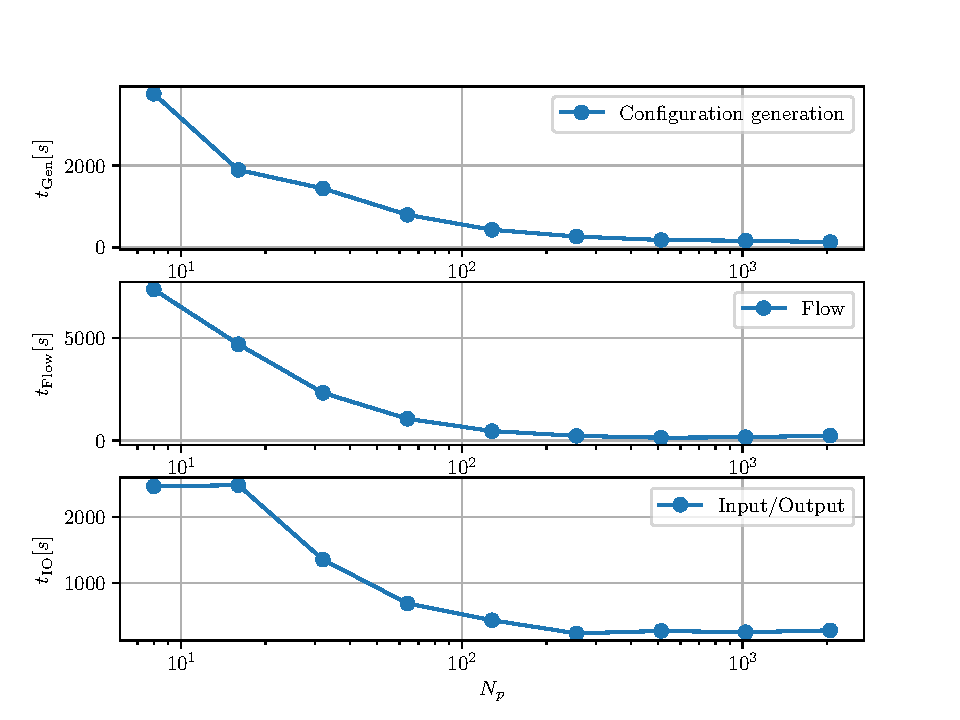
\includegraphics[trim={0.4cm 0.0cm 0.4cm 1.2cm},clip,scale=0.35]{../../LQCD/LatticeAnalyser/figures/scaling/strong/strong_all}\end{center}}
\only<2>{\vspace{-10.0pt}\begin{center}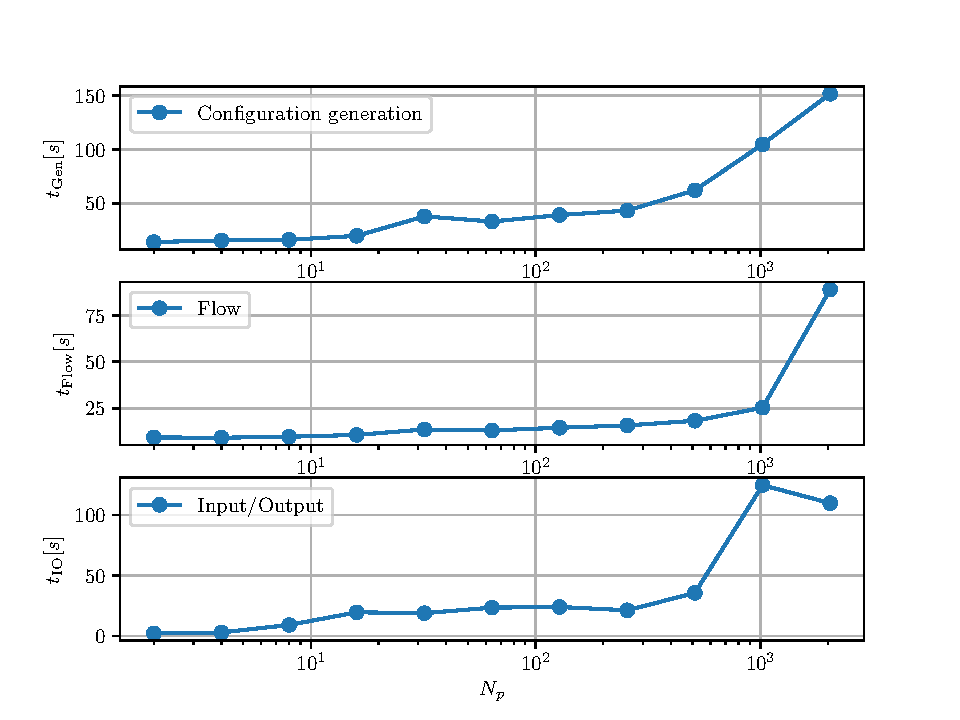
\includegraphics[trim={0.4cm 0.0cm 0.4cm 1.2cm},clip,scale=0.35]{../../LQCD/LatticeAnalyser/figures/scaling/weak/weak_all}\end{center}}
\only<3>{\vspace{-10.0pt}\begin{center}\includegraphics[trim={0.4cm 0.0cm 0.4cm 1.2cm},clip,scale=0.35]{../../LQCD/LatticeAnalyser/figures/scaling/strong/speedup_strong_all}\end{center}}
\only<5>{We appear to have a plateau around 512 cores.}
\note{\begin{itemize}
    \item <1->Strong scaling
    \item <2->Weak scaling
    \item <3->The speedup of the configuration generation, flowing, and IO. The speedup is calculated by dividing the run time of each $N_p$ run, with the run time of the run with the least number of processors, $N_p=8$.
    \item <4->The IO was optimized later to be a factor of ten or more faster.
\end{itemize}}
\end{frame}

\begin{frame}{Optimizing the gauge configuration generation}
\only<1>{Generated 200 configurations for a lattice of size $N^3\times N_T = 16^3 \times 32$ and $\beta=6.0$, for combinations of $N_\mathrm{corr}\in[200,400,600]$ and $N_\mathrm{up}\in[10,20,30]$.}
\only<2>{\begin{center}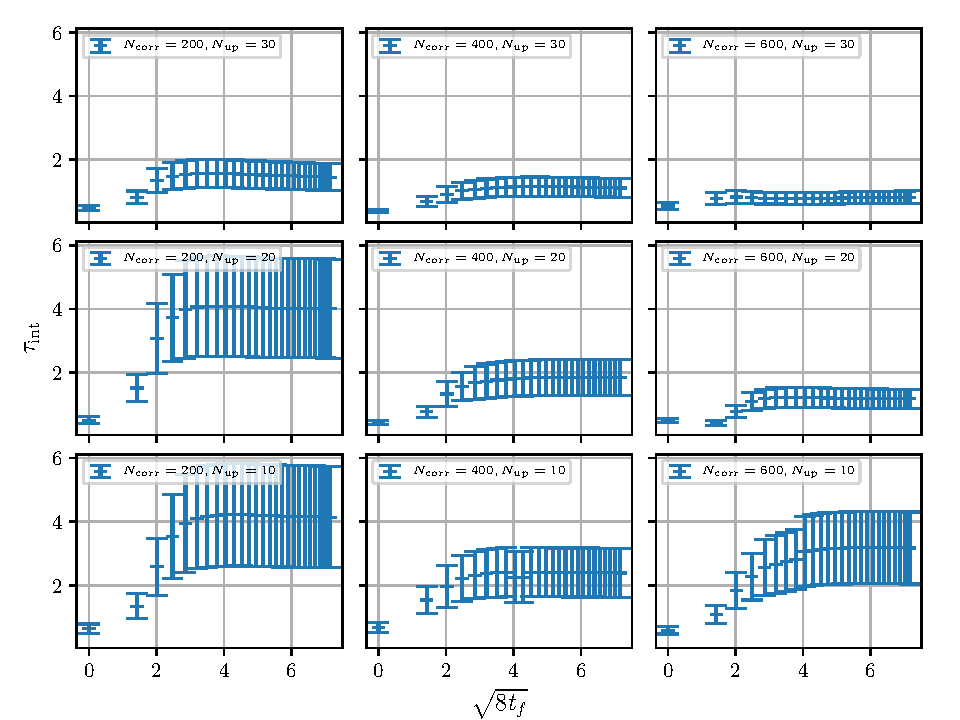
\includegraphics[trim={0.4cm 0.0cm 0.4cm 0.0cm},clip,scale=0.6]{../figures/lattice-updates/topc_autocorr}\end{center}}
\only<3->{\begin{center}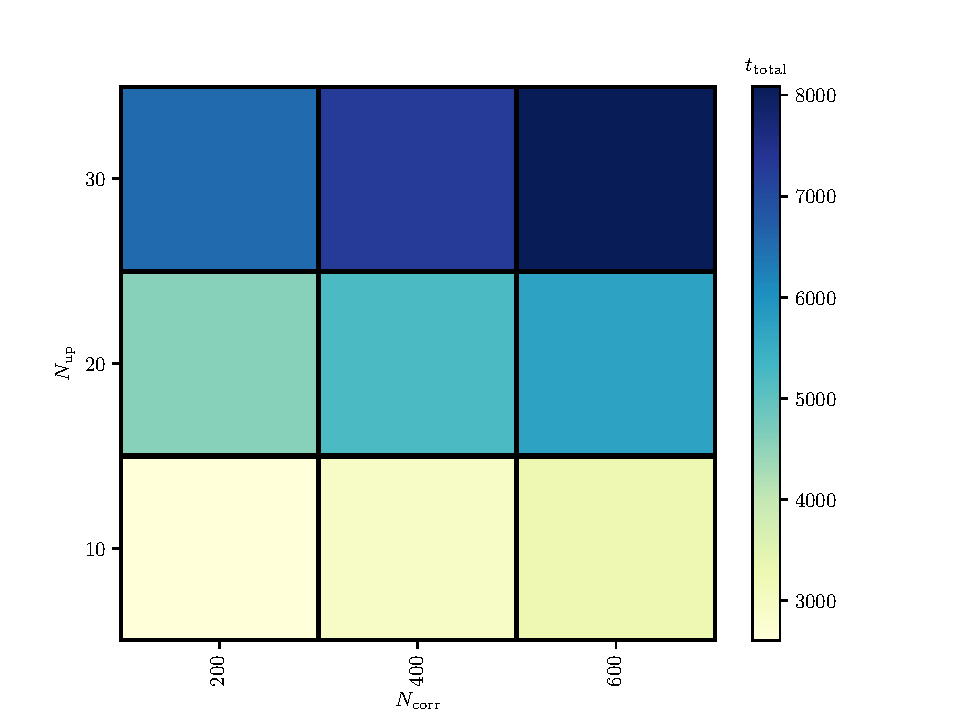
\includegraphics[trim={0.4cm 0.0cm 0.4cm 0.0cm},clip,scale=0.6]{../figures/lattice-updates/topc_total_runtime}\end{center}}
\note{
\begin{itemize}
    \item <1->{We run for different values for $N_\mathrm{up}$ and $N_\mathrm{corr}$ to see what gives optimizes \textbf{computational cost} and \textbf{autocorrelation}.}
    \item <1->{The integrated autocorrelation time for topological charge $\expect{Q}$ for a lattice of size $N=16$ and $N_T=32$ with $\beta=6.0$ for combinations of $N_\mathrm{corr}\in[200,400,600]$ and $N_\mathrm{up}\in[10,20,30]$, plotted against flow time $\sqrt{8t_f}$.}
    \item <2->{The time taking to generate 200 configurations and flowing them $N_\mathrm{flow}=250$ flow steps for a lattice of size $N=16$ and $N_T=32$, with $\beta=6.0$ for combinations of $N_\mathrm{corr}\in[200,400,600]$ and $N_\mathrm{up}\in[10,20,30]$.}
    \item <3->{What we see is that increasing $N_\mathrm{up}$ is a cheaper alternative compared to using $N_\mathrm{corr}$}
\end{itemize}}
\end{frame}

\begin{frame}{Verifying the code}
\begin{itemize}[<+->]
    \item \textbf{Unit testing.} $\SU(3)$, $\SU(2)$ multiplications.
    \item \textbf{Integration testing.} Random matrix generation, lattice objects, parallelization, ect.
    \item \textbf{Validation testing.} Cross checking results with a configuration from Chroma.
\end{itemize}
\end{frame}

\begin{frame}{Additional ensembles}
\begin{table}
    \centering
    \resizebox{0.8\columnwidth}{!}{%
    \begin{tabular}{l r r r r r r r}
        \toprule
        Ensemble & $N$ & $N_T$ & $N_\mathrm{cfg}$ & $N_\mathrm{corr}$ & $N_\mathrm{up}$ & $a$ $[\fm]$ & $L$ $[\fm]$ \\ 
        \midrule
        $E$ & 8 & 16 & 8135 & 600 & 30 & 0.0931(4) & 0.745(3) \\
        $F$ & 12 & 24 & 1341 & 200 & 20 & 0.0931(4) & 1.118(5) \\
        $G$ & 16 & 32 & 2000 & 400 & 20 & 0.0790(3) & 1.265(6) \\
        \bottomrule
    \end{tabular}
    }
\end{table}
\note{\begin{itemize}
    \item Additional ensembles made in order to illuminate additional aspects of the topological charge.
    \item Supporting ensembles made on Smaug. All ensembles were flown $N_\mathrm{flow}=1000$ steps with $\epsilon_\mathrm{flow}=0.01$.
\end{itemize}}
\end{frame}


\end{document}